% !TeX spellcheck = en_GB
\documentclass[main.tex]{subfiles}

\begin{document}
\chapter{Experiments and Discussion}
\lhead{Experiments and Discussion}
\label{chap:discussion}

\section{What Is Going on in the Pretraining?}
\label{sec:pretrainpls}
In order to investigate what affects pretraining effectiveness, several ablation studies are performed.
Unless stated otherwise, the hyperparameters from table \ref{tab:pretrain-hyper} are used, but with 50 epochs due to limited compute.
The experiments were trained primarily on a $ 1\times$A100 configuration.
Due to its negative effect on runtime on A100's (see figure \ref{fig:runtime}), AMP is not used for any of the following experiments.
%TODO Lukas' ting om da-BERTs undertræning. Måske et andet sted end her
\subsection{The Parameter Population}
Figure \ref{fig:weight-dist} shows the distribution before and after pretraining divided by whether or not a given parameter was initialized from da-BERT.
\begin{figure}[H]
    \centering
    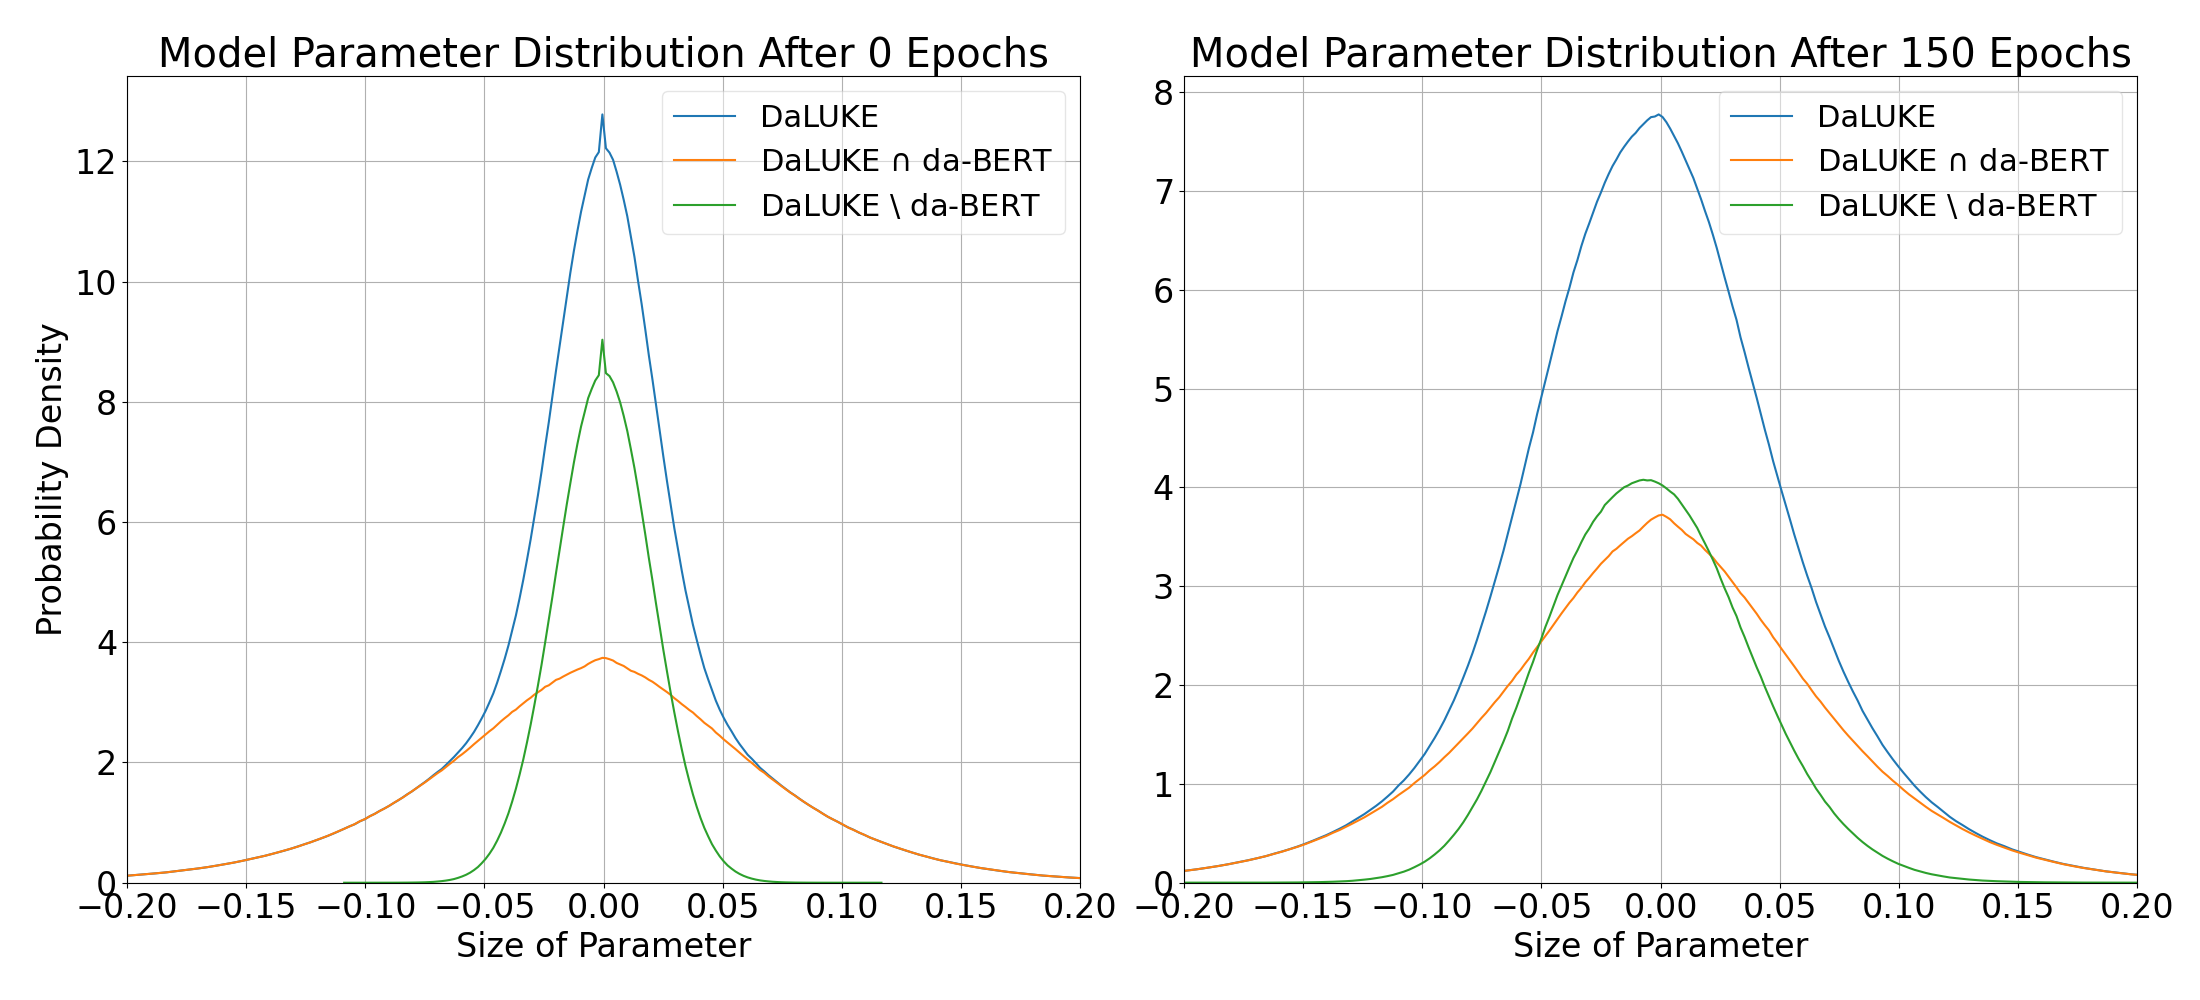
\includegraphics[width=\textwidth]{weights}
    \caption{
        The parameter distribution before and after pretraining.
        The decoder is included but only makes up a relatively small part.
        DaLUKE $ \cap $ da-BERT refers to the parameters that are set in DaLUKE from da-BERT including the query matrices that are strictly not part of da-BERT.
        DaLUKE $ \backslash $ da-BERT are the remaining parameters.
        These are made up of the entity embeddings (58 million parameters) and the entity decoder (58 million parameters).
        In total, the model has 273 million parameters.
        Notetice that DaLUKE $ \cap $ da-BERT and DaLUKE $ \backslash $ da-BERT are not full probability densities but rather subsets that together make up the DaLUKE graph, which is a full probability density.
    }
    \label{fig:weight-dist}
\end{figure}\noindent
Two observations stand out:
Firstly, DaLUKE exclusive parameters, which consist of entity embeddings and the entity part of the decoder, are spread out.
This includes the notable peak that comes from biases and layer normalizations being initialized to 0.
Secondly, the shared parameters are more or less unchanged in their distribution.
This makes sense, as they are already trained, and so further training on similar data with a similar task should not make result in any significant change.
Furthermore, all parameters from da-BERT (barring the three sets of DaLUKE exclusive query matrices) are not changed for the first half of training.
When they are finally unlocked, both the loss and learning rate have dropped significantly resulting in less change.

\subsection{Effect of More Pretraining}
How more pretraining affects the language understanding of the model can be hard to quantify.
Obviously, there is the loss and by extension the top $ k $ accuracy, but these follow directly from the pretraining task and are not direct measures of language understanding.
High scores may also indicate overfitting, especially on small datasets.

One way to glimpse into the pretraining black box is to observe the performance of downstream language tasks on a number of checkpoints produced during the pretraining.
Such a checkpoint was produced just after model initialization and following that after roughly every fifth epoch for a total of 32 checkpoints from the main model.
At every checkpoint, fine-tuning was performed using the hyperparameters from table \ref{tab:baseline-hyper}.
The result is shown in figure \ref{fig:running}.
\begin{figure}[H]
    \centering
    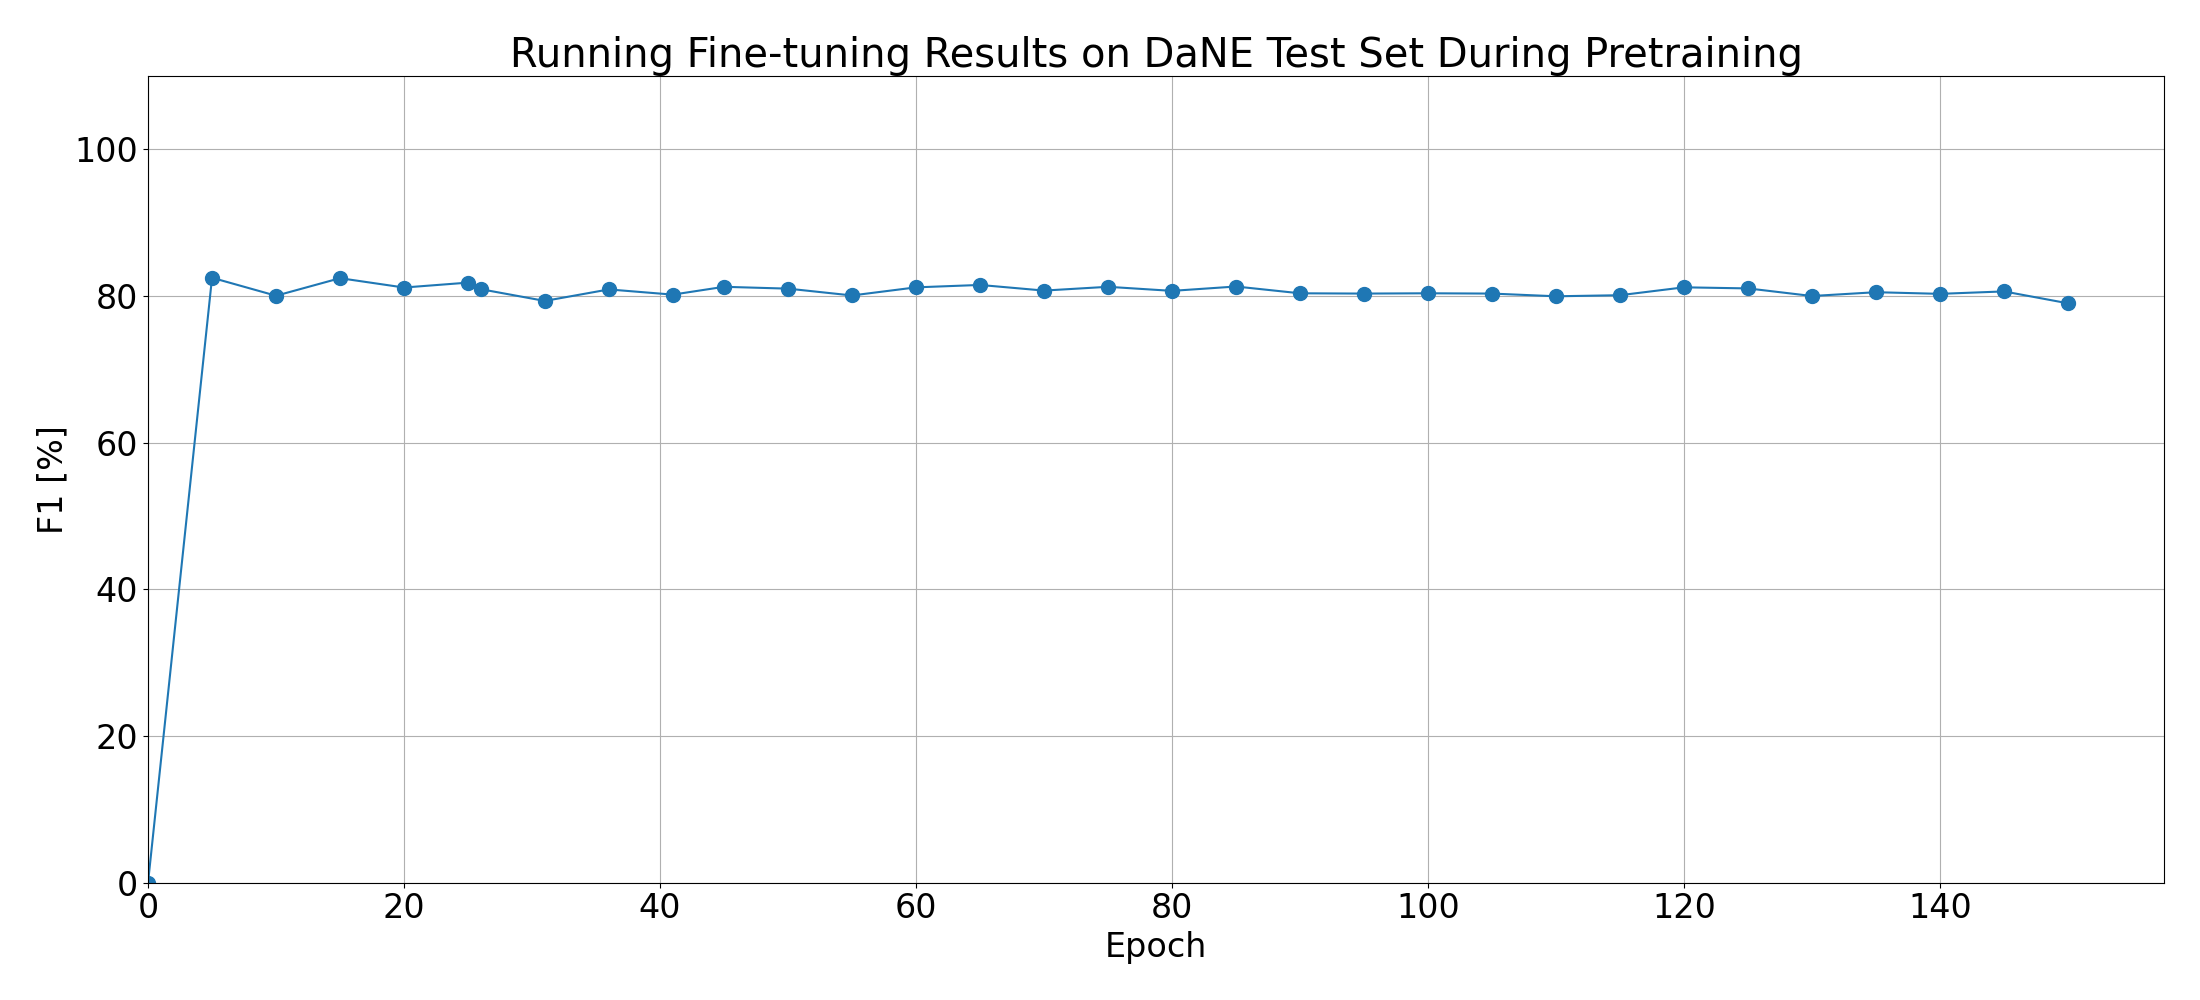
\includegraphics[width=.8\textwidth]{running}
    \caption{Fine-tuning results using different pretraining checkpoints.}
    \label{fig:running}
\end{figure}\noindent
At least for NER, extra pretraining only yields improved results up to five epochs -- or maybe even less, but no checkpoints were saved to test that hypothesis.
After the first five epochs, fine-tuning performance is stagnant.
In fact, the performance curve mirrors that of the masked sub-word accuracy of the MLM (see table \ref{fig:pretrain-acc}).
On the other hand, there is hardly any correlation between the performance and the masked entity accuracy.
This indicates that fine-tuning overwhelmingly relies on the knowledge gained from the BERT part of the model.

\subsection{Baseline}
For a baseline model, the main model is retrained using only 50 epochs, but otherwise using the same hyperparameters, shown in Table \ref{tab:pretrain-hyper}.
This allows for a comparison to a number of ablation studies where compute resources did not allow full 150 epoch pretraining.

The final results of this pretraining are summarized in table \ref{tab:baseline-mlm} with the accuracy development shown on figure \ref{fig:baseline-acc}.

\begin{table}[H]
    \centering
    \small
    \begin{tabular}{l|l|cccccc}
        Model                           & Top $k$ accuracy [\pro]  & $k=1$  & $k=3$ & $k=5$ & $k=10$ & $k=25$ & $k=50$\\\hline
        \multirow{2}{*}{Baseline}       & Masked words             & 24.23  & 30.94 & 34.37 & 39.70  & 47.71  & 53.62 \\
                                        & Masked entities          & 28.80  & 39.01 & 50.64 & 50.64  & 59.57  & 66.32
    \end{tabular}
    \caption{
        The top $k$ accuracy of the baseline model in the 50'th and last epoch.
    }
    \label{tab:baseline-mlm}
\end{table}\noindent
% 2021-06-11 19:37:14.230    INFO        K=1
%                                        Word:   24.231
%                                        Entity: 28.800
% 2021-06-11 19:37:14.235    INFO        K=3
%                                        Word:   30.937
%                                        Entity: 39.009
% 2021-06-11 19:37:14.238    INFO        K=5
%                                        Word:   34.371
%                                        Entity: 43.843
% 2021-06-11 19:37:14.242    INFO        K=10
%                                        Word:   39.701
%                                        Entity: 50.637
% 2021-06-11 19:37:14.245    INFO        K=25
%                                        Word:   47.708
%                                        Entity: 59.567
% 2021-06-11 19:37:14.249    INFO        K=50
%                                        Word:   53.619
%                                        Entity: 66.324
\begin{figure}[H]
    \centering
    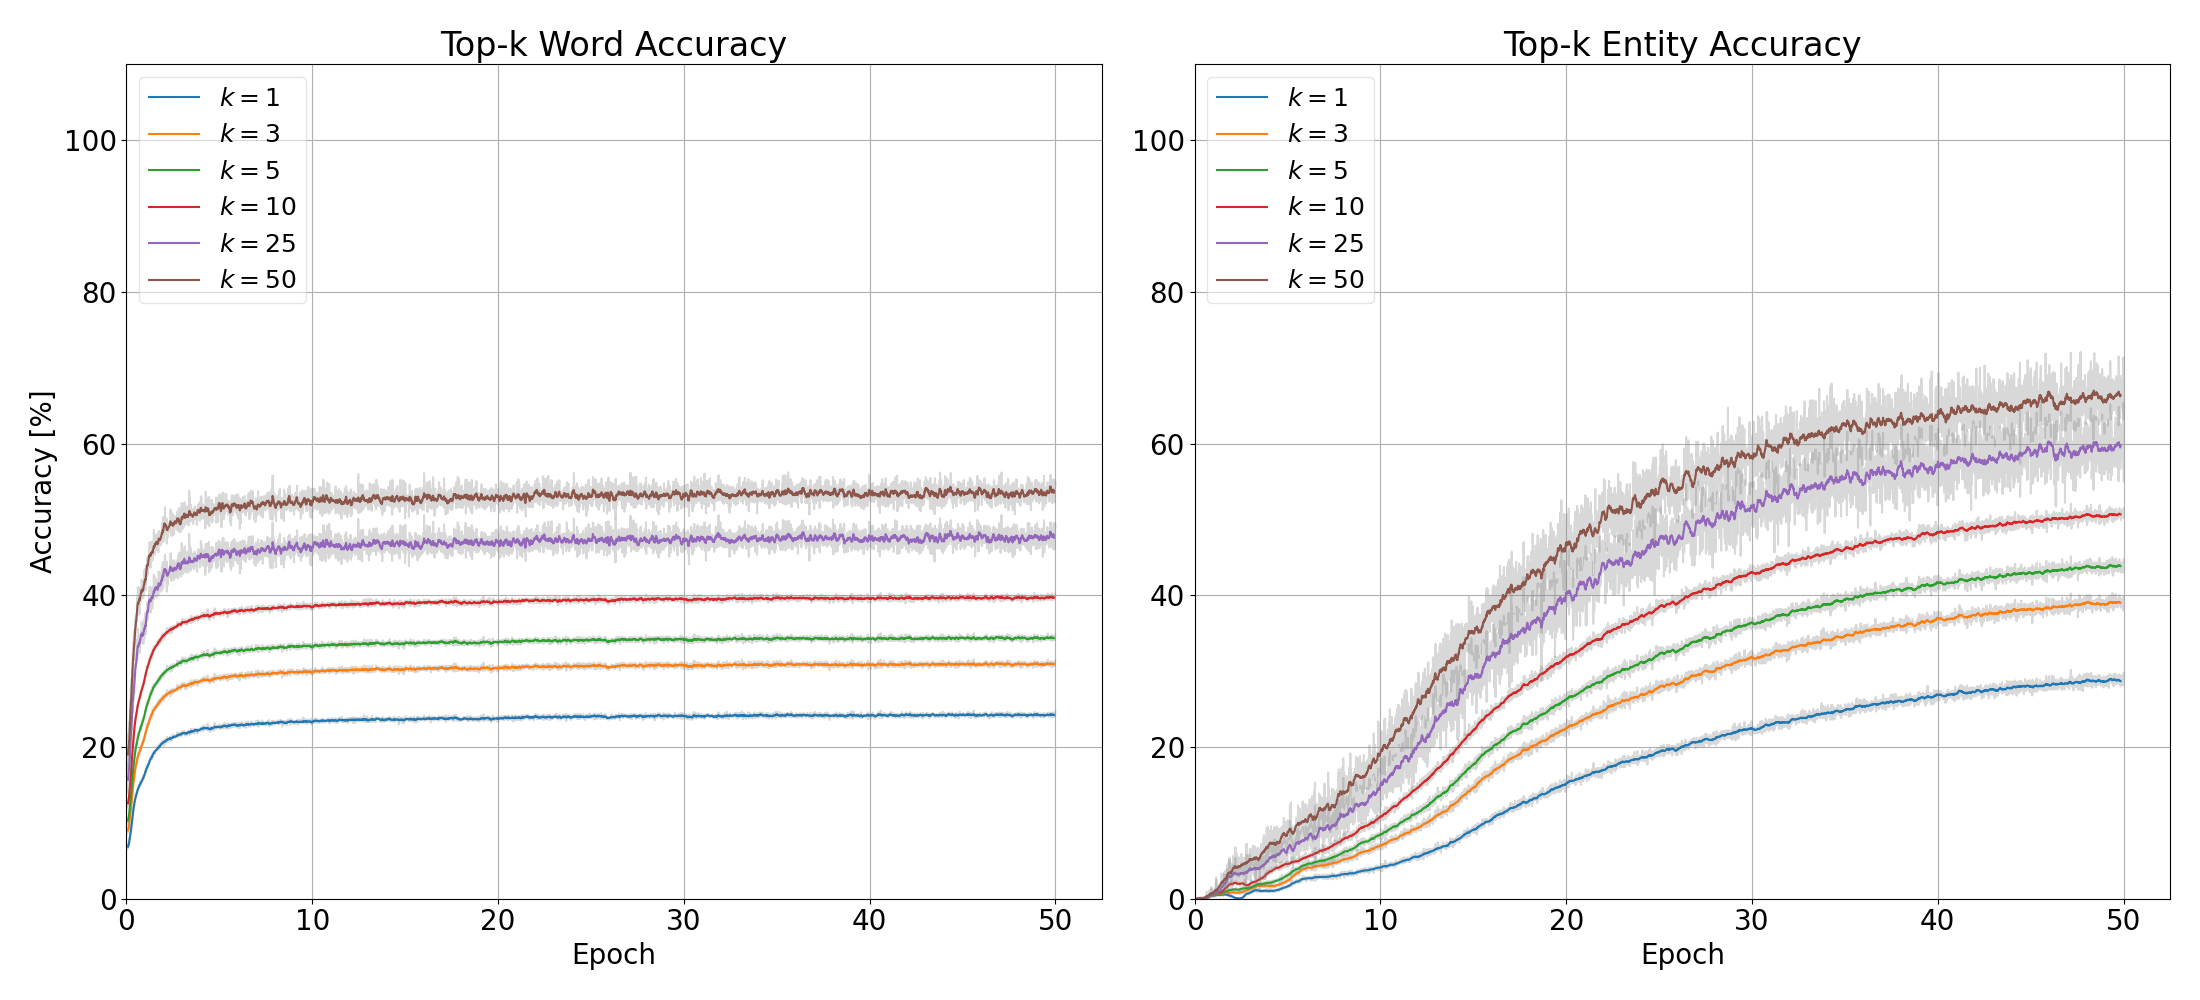
\includegraphics[width=\textwidth]{baseline-acc}
    \caption{Baseline masked language and masked entity accuracy throughout pretraining.}
    \label{fig:baseline-acc}
\end{figure}\noindent
The model is afterwards finetuned for named entity recognition on DaNE following the approach described in Section~\ref{sub:finetune-ner} and the following hyperparameters, non-systematically selected:
\begin{table}[H]
    \centering
    \small
    \begin{tabular}{l|r}
        Parameter  &    \jl{Value}\\\hline
        Epochs     & 10\\
        Batch size &    16\\
        Peak learning rate & $2\ctp{-5}$\\
        LR warmup steps proportion & $ 6\pro $\\
        Dropout (pretrained model) & $ 0.1 $\\
        Dropout (final, linear layer) & $ 0.025 $\\
        Weight decay & $ 0.05 $\\
        Loss weighting & No
    \end{tabular}
    \caption{Hyperparameters for baseline finetuning experiment and the following ablation experiments.}\label{tab:baseline-hyper}
\end{table}\noindent
This resulted in the following performance on the DaNE test data-set.
\begin{table}[H]
    \centering
    \small
    \begin{tabular}{l|ccccc|c|c}
        \multirow{2}{*}{Model}  & \multicolumn{5}{c|}{F1 [\pro]} & Precision [\pro]               & Recall [\pro]               \\
                            & Avg. & LOC & PER & ORG & MISC      & Avg.                           & Avg.                         \\ \hline
    Baseline                & 82.41&89.58&92.90&74.48&68.84      & 86.73                          & 78.49
    \end{tabular}
    \caption{The baseline finetuning results where avg. refers to the micro average}
    \label{tab:summary}
\end{table}\noindent
The results of the baseline experiment together with the following experiments are also shown together in a final overview at Section \ref{subsec:preoverview}.
 % 2021-06-11 19:53:46.665    INFO                      precision    recall f1-score   support

 %                                                LOC     0.8958    0.8958   0.8958        96
 %                                               MISC     0.7872    0.6116   0.6884       121
 %                                                ORG     0.8372    0.6708   0.7448       161
 %                                                PER     0.9140    0.9444   0.9290       180

 %                                          micro avg     0.8673    0.7849   0.8241       558
 %                                          macro avg     0.8586    0.7807   0.8145       558
 %                                       weighted avg     0.8612    0.7849   0.8180       558

\subsection{Dataset Augmentation}

\ref{tab:metadata}
A key addition to the pretraining pipeline was the addition of extra entity annotations not already in the Wikipedia articles themselves using pattern matching as explained in Section~\ref{subsec:entaug}.
This resulted in a 47\pro\ growth in the number of annotations as shown in Table~\ref{tab:metadata}.
While it was argued that it should improve performance, it was all theoretical.
Therefore, this effect of the augmentation is investigated by pretraining a model with the original data for 50 epochs and same hyperparameters as the main experiment.

The pretraining terminated to the following performance.

\begin{table}[H]
    \centering
    \small
    \begin{tabular}{l|l|cccccc}
        Model                               & Top $k$-accuracy [\pro]  & $k=1$  & $k=3$ & $k=5$ & $k=10$ & $k=25$ & $k=50$\\\hline
        \multirow{2}{*}{No data aug.}       & Masked words             & 25.26  & 32.16 & 35.60 & 40.93  & 48.78  & 54.62 \\
                                            & Masked entities          & 34.02  & 42.85 & 47.21 & 53.52  & 62.26 & 68.82
    \end{tabular}
    \caption{
        The top $k$ accuracy of the pretrained model trained without dataset augmentation in the 50'th and last epoch.
    }
    \label{tab:old-data-mlm}
\end{table}
At a first glance, these masked language modelling results that strictly dominate the numbers for the baseline seems to suggest that the dataset augmentation was ill-advised.
There is, however, a large issue (apart from the obvious problem of judging a model by it's performance on the training data set) with the metric in this case:
The dataset augmentation also changed the benchmark itself as the masking task of the baseline model also includes automatically annotated, and thus somewhat dubious, entity links.
This can explain the clear gain in entity masking performance.
Whether this explanation has any merit in explaining the increased word accuracy found in this ablation study is less clear to us and relates to the model synergy effects in this joint task.

% 2021-06-11 19:38:23.333    INFO        K=1
%                                        Word:   25.260
%                                        Entity: 34.015
% 2021-06-11 19:38:23.340    INFO        K=3
%                                        Word:   32.155
%                                        Entity: 42.846
% 2021-06-11 19:38:23.345    INFO        K=5
%                                        Word:   35.601
%                                        Entity: 47.212
% 2021-06-11 19:38:23.351    INFO        K=10
%                                        Word:   40.926
%                                        Entity: 53.520
% 2021-06-11 19:38:23.356    INFO        K=25
%                                        Word:   48.776
%                                        Entity: 62.258
% 2021-06-11 19:38:23.361    INFO        K=50
%                                        Word:   54.617
%                                        Entity: 68.818
As a more unbiased benchmark, this model was finetuned on the DaNE data set using the hyperparameters at Table~\ref{tab:baseline-hyper} resulting in the following performance:
\begin{table}[H]
    \centering
    \small
    \begin{tabular}{l|ccccc|c|c}
        \multirow{2}{*}{Model}  & \multicolumn{5}{c|}{F1 [\pro]} & Precision [\pro]               & Recall [\pro]               \\
                            & Avg. & LOC & PER & ORG & MISC      & Avg.                           & Avg.                         \\ \hline
    No data aug.            & 83.07&84.42&95.18&76.41&72.10      & 85.42                          & 80.82
    \end{tabular}
    \caption{The finetuning results of the dataset augmentation pretraining experiment.}
    \label{tab:dataaug}
\end{table}
% 2021-06-11 16:08:34.724    INFO                      precision    recall  f1-score   support

%                                                 LOC     0.8155    0.8750    0.8442        96
%                                                MISC     0.7500    0.6942    0.7210       121
%                                                 ORG     0.8214    0.7143    0.7641       161
%                                                 PER     0.9711    0.9333    0.9518       180

%                                           micro avg     0.8542    0.8082    0.8306       558
%                                           macro avg     0.8395    0.8042    0.8203       558
%                                        weighted avg     0.8532    0.8082    0.8291       558
The ablation study gets substantially higher recall than the baseline resulting in a higher micro average F1 score on the NER task, though the baseline outperforms in precision.

All in all, these benchmarks cannot be used to argue that the theorized problem of of false negatives in the volunteer-produced annotations is mitigated by this augmentation approach resulting in a better language understanding.
If anything, the addition of automatic pattern-matched annotations worsened the performance slightly.

As the addition of these $47\pro$ bronze standard annotations did directly stop the learning, we still propose this approach as an avenue for further development of DaLUKE.
Much needed entirely new LUKE pretraining data sets could be produced from raw text corpora by automatically annotating them using pattern matching.
Such lower standard annotations used to achieve extra data might be necessary for continued improvement in low-resource languages such as Danish but should be used carefully and with an analysis of the trade off between quality and quantity of data.

\subsection{Entity-aware Self-attention}
One of Yamada et al.'s key contributions to the transformer is the addition of query matrices for relations between entities and words.
They do not use these extra matrices in the pretraining but instead let them be learned during downstream tasks, initializing them to the word-to-word matrices of RoBERTa.
They perform ablation studies on multiple datasets, showing an improvement in every case over original attention.
\cite{yamada2020luke}

These results suggest that training the extra query matrices in the pretraining also might have a positive impact.
For this reason, entity-aware self-attention has been used here for all pretrainings bar this one, where its effects on pretraining is investigated.

\begin{table}[H]
    \centering
    \small
    \begin{tabular}{l|l|cccccc}
        Model                               & Top $k$-accuracy [\pro]  & $k=1$  & $k=3$ & $k=5$ & $k=10$ & $k=25$ & $k=50$\\\hline
        \multirow{2}{*}{BERT attention}     & Masked words             & 20.63  & 26.29 & 29.41 & 34.58  & 42.44  & 48.73 \\
                                            & Masked entities          & 12.26  & 20.98 & 25.69 & 32.76  & 42.88 & 51.52
    \end{tabular}
    \caption{
        The top $k$ accuracy of the pretrained model trained without entity-aware self-attention in the 50'th and last epoch.
    }
    \label{tab:bert-attention-mlm}
\end{table}\noindent
After finetuning, the following results were achieved:

\begin{table}[H]
    \centering
    \small
    \begin{tabular}{l|ccccc|c|c}
        \multirow{2}{*}{Model}  & \multicolumn{5}{c|}{F1 [\pro]} & Precision [\pro]               & Recall [\pro]               \\
                            & Avg. & LOC & PER & ORG & MISC      & Avg.                           & Avg.                         \\ \hline
    BERT attention          & 79.62 & 85.86 & 92.84 & 70.95 &   64.84      & 84.51                          & 75.27
    \end{tabular}
   \caption{The finetuning results of the traditional attention experiment.}
    \label{tab:bertatt}
\end{table}

% 2021-06-12 12:21:29.881    INFO                      precision    recall  f1-score   support

%                                                 LOC     0.7191    0.6667    0.6919        96
%                                                MISC     0.6585    0.4463    0.5320       121
%                                                 ORG     0.6364    0.2609    0.3700       161
%                                                 PER     0.7563    0.5000    0.6020       180

%                                           micro avg     0.7022    0.4480    0.5470       558
%                                           macro avg     0.6926    0.4685    0.5490       558
%                                        weighted avg     0.6941    0.4480    0.5354       558
\begin{enumerate}
    \item Performance og træningskurver uden entity-aware attention
%    \item Køretidssammenligning på de to modeller
\end{enumerate}

\subsection{Impact of Danish BERT}
As described in section \ref{sec:LUKE}, many of the weights are initialized from a base transformer.
This transfer step ideally gives DaLUKE all the contextual language understanding of da-BERT without having to learn it all.
In order to test this hypothesis, a pretraining is conducted without initializing the weights to da-BERT.

\begin{table}[H]
    \centering
    \small
    \begin{tabular}{l|l|cccccc}
        Model                                 & Top $k$ accuracy [\pro]  & $k=1$  & $k=3$ & $k=5$ & $k=10$ & $k=25$ & $k=50$\\\hline
        No transfer & Masked words             & 47.86  & 59.28 & 63.92 & 69.83  & 76.51  & 81.04 \\
        learning                                      & Masked entities          & 81.71  & 87.19 & 88.87 & 90.90  & 93.15 & 94.56
    \end{tabular}
    \caption{
        The top $K$ accuracy of the pretrained model trained without initializing weights from da-BERT in the 50'th and last epoch.
    }
    \label{tab:nobert-mlm}
\end{table}\noindent
It is immediately clear from table \ref{tab:nobert-mlm} that this model performs noticably better at both the masked word and masked entity tasks than other models so far.
That is despite even starting from 0 in the masked word task (see figure \ref{fig:nobert-acc}).
Because of this, good NER performance could reasonbly be expected.
This did not happen - in fact, results were much worse than the baseline.
% 2021-06-12 12:20:54.130    INFO                      precision    recall  f1-score   support

%                                                 LOC     0.7281    0.8646    0.7905        96
%                                                MISC     0.6514    0.5868    0.6174       121
%                                                 ORG     0.7841    0.4286    0.5542       161
%                                                 PER     0.8683    0.8056    0.8357       180

%                                           micro avg     0.7699    0.6595    0.7104       558
%                                           macro avg     0.7580    0.6714    0.6995       558
%                                        weighted avg     0.7728    0.6595    0.6994       558

\begin{table}[H]
    \centering
    \small
    \begin{tabular}{l|ccccc|c|c}
        \multirow{2}{*}{Model}  & \multicolumn{5}{c|}{F1 [\pro]} & Precision [\pro]               & Recall [\pro]               \\
                            & Avg. & LOC & PER & ORG & MISC      & Avg.                           & Avg.                         \\ \hline
    No transfer learning    & 71.04&79.05&83.57&55.42&61.74      & 76.99                          & 65.95
    \end{tabular}
    \caption{The finetuning results of the experiment where weights were trained from scratch}
    \label{tab:nobert}
\end{table}
\begin{figure}[H]
    \centering
    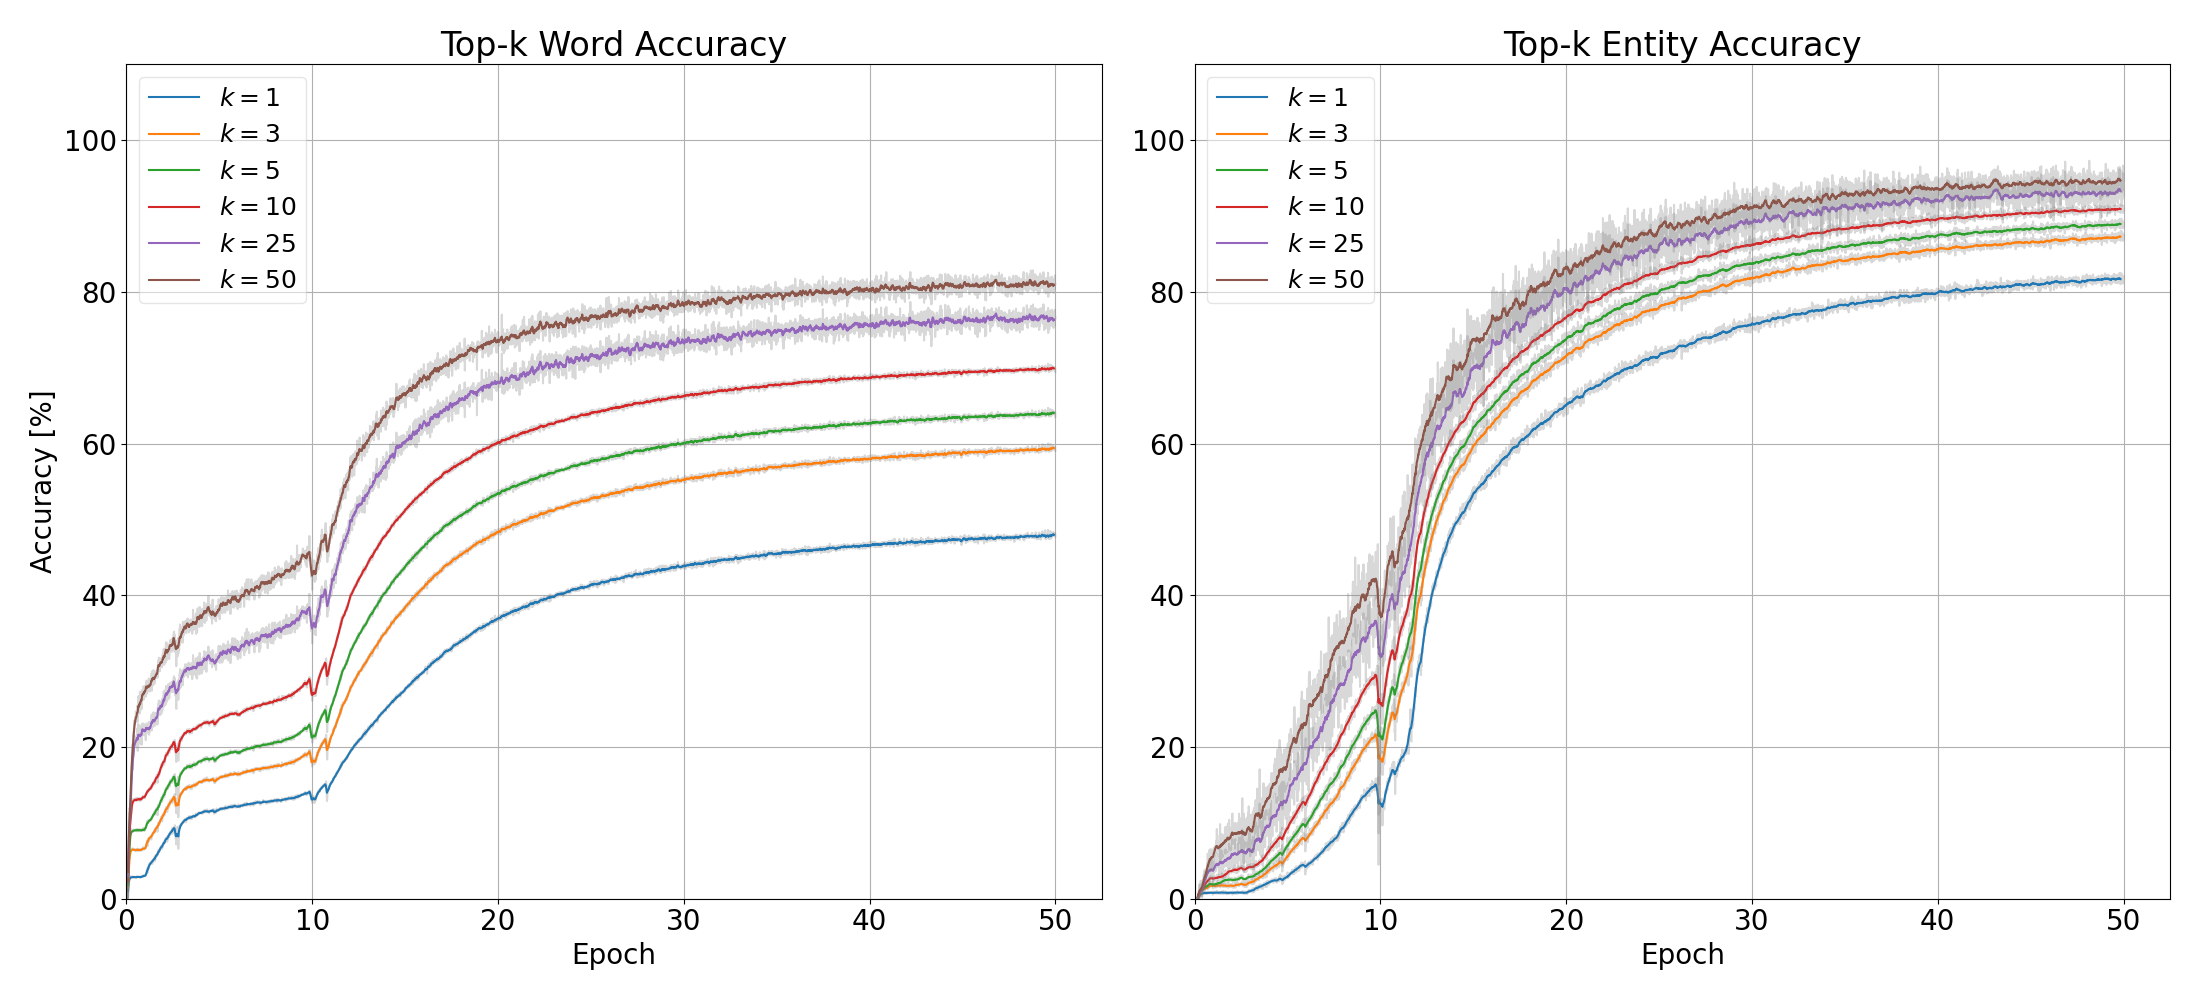
\includegraphics[width=\linewidth]{nobert-acc.png}
    \caption{Development of the masked word and entity accuracies during the course of the pretraining without initializing from da-BERT weights.
    All curves are smoothed using a rolling average.}
    \label{fig:nobert-acc}
\end{figure}\noindent
The transfer learning from da-BERT clearly turns out to be a help here.
From figure \ref{fig:nobert-acc}, the initialization seems to provide two things other than initial MLM accuracy:
\begin{itemize}
    \item A regulazation effect that prevents the model from overfitting to the dataset.
    \item Increased pretraining stability.
    The accuracy curves contain a number of sudden jumps and drops that are much rarer in other pretrainings.
\end{itemize}
It should be noted that because no weights came from da-BERT, no weights were ever locked throughout pretraining.
A similar experiment with weights unlocked and initialization from da-BERT showed pretraining accuracies much closer to the baseline, indicating that the regualizing effect is indeed da-BERT.
%TODO Under-undereksperimentet skal måske formaliseres mere

\begin{enumerate}
    \item Performance og træningskurver for eksperimentet, hvor BERT-vægte ikke bruges
    \item Her rapporteres under-eksperimentet med performance for da-BERT på vores datasæt
    \item Her kan henvises til parameterplotsene i en diskussion af BERT-vægtenes rolle
\end{enumerate}

\subsection{Entity Vocabulary Size}
For the English LUKE, Yamada et al. used an entity vocabulary of the $500\ctp3$ entities \cite[Sec. 3.4]{yamada2020luke} even though the English Wikipedia contains $\sim 6\ctp6$ content pages\footnotemark.
\footnotetext{English Wikipedia Statistics: \url{https://en.wikipedia.org/wiki/Special:Statistics}. Visited March 3, 2021.}
This is, apart from crude filtering of non-entity pages, a result of cutting the entity domain down to the most frequent hyperlinks.
For the Danish Wikipedia, however, the number of content pages is $\sim 267\ctp3$ \footnotemark resulting in the DaLUKE entity vocabulary containing $\sim 225\ctp3$ entities.
\footnotetext{Danish Wikipedia Statistics: \url{https://da.wikipedia.org/wiki/Speciel:Statistik} Visited March 3, 2021.}
As this is a much smaller world of entities, the entity vocabulary of the main DaLUKE model was not cut by frequency.

An experiment was performed where entities that were mentioned less than 50 times were excluded from the data, resulting in a vocabulary of $19,119$ entities.
This was done on the augmented data explained in Section \ref{sec:dawiki}.
After pretraining for 50 epochs with the same hyperparameters as the main experiment, the following performance was observed.

\begin{table}[H]
    \centering
    \small
    \begin{tabular}{l|l|cccccc}
        Model                                 & Top $k$-accuracy [\pro]  & $k=1$  & $k=3$ & $k=5$ & $k=10$ & $k=25$ & $k=50$\\\hline
        \multirow{2}{*}{Limited entity vocab.}& Masked words             & 23.91  & 30.50 & 33.90 & 39.19  & 47.11  & 53.03 \\
                                              & Masked entities          & 30.56  & 42.15 & 48.87 & 55.79  & 65.91  & 66.32
    \end{tabular}
    \caption{
        The top $k$ accuracy of the entity vocabulary-limited model in the 50'th and last epoch.
    }
    \label{tab:few-ents-acc}
\end{table}\noindent
The performance on the word prediction task is slightly worse for this entity vocabulary experiment, while clearly higher scores are seen on the masked entity task.
As for the data augmentation experiment, attention must again be put on the changes in the benchmark itself as the accuracy of 31\pro in calculated in a $\sim 20\ctp3$ class problem while the baseline accuracy of 29\pro is calculated over almost ten times as many classes.

% 2021-06-11 19:38:47.989    INFO        K=1
%                                        Word:   23.905
%                                        Entity: 30.585
% 2021-06-11 19:38:47.998    INFO        K=3
%                                        Word:   30.500
%                                        Entity: 42.149
% 2021-06-11 19:38:48.005    INFO        K=5
%                                        Word:   33.902
%                                        Entity: 47.872
% 2021-06-11 19:38:48.011    INFO        K=10
%                                        Word:   39.185
%                                        Entity: 55.786
% 2021-06-11 19:38:48.017    INFO        K=25
%                                        Word:   47.108
%                                        Entity: 65.914
% 2021-06-11 19:38:48.022    INFO        K=50
%                                        Word:   53.028
%                                        Entity: 73.347

The NER performance of this model was, following the approach in the previous experiments, found to be quite close to the performance of the baseline with an average F1 0.2\pro\ points worse.

\begin{table}[H]
    \centering
    \small
    \begin{tabular}{l|ccccc|c|c}
        \multirow{2}{*}{Model}  & \multicolumn{5}{c|}{F1 [\pro]} & Precision [\pro]               & Recall [\pro]               \\
                            & Avg. & LOC & PER & ORG & MISC      & Avg.                           & Avg.                         \\ \hline
    Limited entity vocab.   & 82.22&89.69&93.59&74.00&68.72      & 85.02                          & 79.57
    \end{tabular}
    \caption{The finetuning results of the entity vocabulary limiting pretraining experiment.}
    \label{tab:ent-limit}
\end{table}
% 2021-06-11 15:26:30.316    INFO                      precision    recall  f1-score   support

%                                                 LOC     0.8878    0.9062    0.8969        96
%                                                MISC     0.7358    0.6446    0.6872       121
%                                                 ORG     0.7986    0.6894    0.7400       161
%                                                 PER     0.9385    0.9333    0.9359       180

%                                           micro avg     0.8506    0.7957    0.8222       558
%                                           macro avg     0.8402    0.7934    0.8150       558
%                                        weighted avg     0.8455    0.7957    0.8188       558

Conclusively, the results of this experiment are close to the baseline, signifying robustness in the approach.
However, with these hyperparameters, the removal of entities does not seem promising for the Danish data set.

This experimental filtering of the DaLUKE entities preserves $7\pro$ of the content pages, while $8\pro$ were preserved for the English LUKE.
Intuitively, it would make sense that the same proportional filtering works better in English, as the absolute number of entities making up the implicit knowledge base of the model might be important:
Smaller datasets, corresponding to smaller language areas, do not equate a smaller shared world of named entities.

This conceptual argument somewhat supported by the experimental results suggests that more of the rare entities should be included when working with smaller datasets, though a more continuous experimental search of this filtering parameter might yield a better trade-off than our main model solution of including all entities.

\subsection{Summary} \label{subsec:preoverview}

\begin{table}[H]
    \centering
    \footnotesize
    \begin{tabular}{l|l|cccccc}
        Model                                 & Top $k$-accuracy [\pro]  & $k=1$  & $k=3$ & $k=5$ & $k=10$ & $k=25$ & $k=50$\\\hline
        \multirow{2}{*}{Baseline}             & Masked words             & 24.23  & 30.94 & 34.37 & 39.70  & 47.71  & 53.62 \\
                                              & Masked entities          & 28.80  & 39.01 & 50.64 & 50.64  & 59.57  & 66.32 \\\hline
        \multirow{2}{*}{No data aug.}         & Masked words             & \underline{25.26}  & \underline{32.16} & \underline{35.60} & \underline{40.93}  & \underline{48.78}  & \underline{54.62} \\
                                              & Masked entities          & \underline{34.02}  & 42.85 & 47.21 & 53.52  & 62.26 & \underline{68.82} \\\hline
        \multirow{2}{*}{BERT attention}       & Masked words             & 20.63  & 26.29 & 29.41 & 34.58  & 42.44  & 48.73 \\
                                              & Masked entities          & 12.26  & 20.98 & 25.69 & 32.76  & 42.88 & 51.52 \\\hline
        \multirow{2}{*}{No transfer learning} & Masked words             & \bfseries 47.86  & \bfseries 59.28 & \bfseries 63.92 & \bfseries 69.83  & \bfseries 76.51  & \bfseries 81.04 \\
                                              & Masked entities          & \bfseries 81.71  & \bfseries 87.19 & \bfseries 88.87 & \bfseries 90.90  & \bfseries 93.15 & \bfseries 94.56 \\\hline
        \multirow{2}{*}{Limited entity vocab.}& Masked words             & 23.91  & 30.50 & 33.90 & 39.19  & 47.11  & 53.03 \\
                                              & Masked entities          & 30.56  & \underline{42.15} & \underline{48.87} & \underline{55.79}  & \underline{65.91}  & 66.32
    \end{tabular}
    \caption{
        Overview of final pretraining results for all the experiments presented previously.
        Best result for each metric is shown in boldface with second best result underlined (motivated by quite boring distribution of bests).
    }
    \label{tab:mlmsummary}
\end{table}

\begin{table}[H]
    \centering
    \footnotesize
    \begin{tabular}{l|ccccc|c|c}
        \multirow{2}{*}{Model}  & \multicolumn{5}{c|}{F1 [\pro]} & Precision [\pro]               & Recall [\pro]               \\
                            & Avg. & LOC & PER & ORG & MISC      & Avg.                           & Avg.                        \\ \hline
    Baseline                & 82.41&89.58&92.90&74.48&68.84      & \textbf{86.73}                          & 78.49                       \\
    No data augmentation    & \textbf{83.07}&84.42&\textbf{95.18}&\textbf{76.41}&\textbf{72.10}      & 85.42                          & \textbf{80.82}                       \\
    BERT attention          & 79.62 & 85.86 & 92.84 & 70.95 &   64.84      & 84.51                          & 75.27 \\
    No transfer learning    & 71.04&79.05&83.57&55.42&61.74      & 76.99                          & 65.95                       \\
    Limited entity vocab.   & 82.22&\textbf{89.69}&93.59&74.00&68.72      & 85.02                          & 79.57
    \end{tabular}
    \caption{Overview of the pretraining experiment finetuning results presented in the previous subsections.}
    \label{tab:nersummary}
\end{table}

\section{Finetuning Performance}
\label{sec:finetuning-exp}
\begin{enumerate}
    \item Statistiske metoder til sammenligning af scores (????)
    \item Prec. vs rec. - bør måske være i 6.3, da det jo er mere analyse-agtigt?
%    \item Gør det klart, at alle bruger den store Carlos
    \item Gør det klart, hvad baseline er
\end{enumerate}
As with pretraining, fine-tuning has a number of interesting elements that are worth investigating further.
For these experiments, the main pretrained model from section \ref{sec:Pretraining of daLUKE} are used but with the optimized fine-tuning hyperparameters from table \ref{tab:main-hyper}.
Following the pretraining experiments, all results are reported with MISC.
\subsection{Stability of LUKE Finetuning}

\subsubsection{Reproducability of English LUKE}
For the reproduction of the English LUKE, the results were initially underwhelming as five repetitions of the finetuning of LUKE large on CoNLL2003 consistently, slightly underperformed the reported result of 94.3\pro\ micro average as seen at table \ref{tab:EnLUKE-wrong}.
After investigating, this somewhat disappointing result was revealed to be overturned when finetuning with Python version 3.6 and PyTorch 1.2 instead of using newer versions as done in the initial run.
Using these correct versions, the same as Yamada et al. reported in their package file, the results were succesfully reproduced as shown in the central results in Section \ref{sec:English LUKE Reproduction}.
For the large model, only one of the five repetitions yielded the reported performance.
No criticism can be raised based on this results; the sample size is small and, furthermore, we found that the mean \emph{base} model performance superseded the reported micro average F1 score of 93.3\pro.

All in all, the slight hiccups in reproducing the finetuning results show the difficulties in empiric evaluations of deep methods strongly relying on indeterminism -- especially as the underlying framework, PyTorch, does not guarantee reproducable results across versions and platforms, even if using identical seeds for the random number generator \cite{pytorchrep}.

\begin{table}[H]
    \centering
    \small
    \begin{tabular}{l r r r r r}
            Model & Micro avg. & LOC & PER & ORG & MISC \\
            \hline
            LUKE large & $93.97 \pm  0.07$ & $95.06 \pm  0.2$ & $97.19 \pm  0.08$ & $93.51 \pm  0.2$ & $85.15 \pm  0.4$ \\
                &  &  &  &  &  \\
            Support & 5616 & 1666 & 1602 & 1647 & 701 \\
    \end{tabular}
    \caption{
        Results when pre-training and evaluating LUKE with Python version 3.8 and PyTorch 1.4.
        Values are mean and standard deviance of F1 scores over five repetitions of the fine-tuning.
    }
    \label{tab:EnLUKE-wrong}
\end{table}

\subsubsection{Randomness of DaLUKE Results}
\paragraph{Random number generation variance}

The same repetition of the finetuning procedure as carried out for English LUKE is done for the main DaLUKE pretrained model by training with five different random number generation (RNG) seeds.
The results are shown in table \ref{tab:seeds}.

              % precision    recall  f1-score   support

         % LOC     0.8632    0.8542    0.8586        96
        % MISC     0.8370    0.6364    0.7230       121
         % ORG     0.8417    0.7267    0.7800       161
         % PER     0.9651    0.9222    0.9432       180

   % micro avg     0.8876    0.7921    0.8371       558
   % macro avg     0.8767    0.7849    0.8262       558
% weighted avg     0.8842    0.7921    0.8338       558

              % precision    recall  f1-score   support

         % LOC     0.7963    0.8958    0.8431        96
        % MISC     0.7890    0.7107    0.7478       121
         % ORG     0.8015    0.6522    0.7192       161
         % PER     0.9222    0.9222    0.9222       180

   % micro avg     0.8390    0.7939    0.8158       558
   % macro avg     0.8273    0.7952    0.8081       558
% weighted avg     0.8368    0.7939    0.8122       558

              % precision    recall  f1-score   support

         % LOC     0.8776    0.8958    0.8866        96
        % MISC     0.7963    0.7107    0.7511       121
         % ORG     0.8264    0.7391    0.7803       161
         % PER     0.9438    0.9333    0.9385       180

   % micro avg     0.8693    0.8226    0.8453       558
   % macro avg     0.8610    0.8198    0.8391       558
% weighted avg     0.8665    0.8226    0.8433       558
              % precision    recall  f1-score   support

         % LOC     0.7961    0.8542    0.8241        96
        % MISC     0.7727    0.7025    0.7359       121
         % ORG     0.7801    0.6832    0.7285       161
         % PER     0.9535    0.9111    0.9318       180

   % micro avg     0.8384    0.7903    0.8137       558
   % macro avg     0.8256    0.7877    0.8051       558
% weighted avg     0.8372    0.7903    0.8121       558

              % precision    recall  f1-score   support

         % LOC     0.8454    0.8542    0.8497        96
        % MISC     0.7925    0.6942    0.7401       121
         % ORG     0.7823    0.7143    0.7468       161
         % PER     0.9432    0.9222    0.9326       180

   % micro avg     0.8498    0.8011    0.8247       558
   % macro avg     0.8408    0.7962    0.8173       558
% weighted avg     0.8473    0.8011    0.8230       558
\begin{table}[H]
    \centering
    \begin{tabular}{l|ccccc|c|c}
        \multirow{2}{*}{Seed}  & \multicolumn{5}{c|}{F1 [\pro]} & Precision [\pro]               & Recall [\pro]               \\
                            & Avg. & LOC & PER & ORG & MISC      & Avg.                           & Avg.                        \\ \hline
     1                      & 83.71&85.86&94.32&78.00&72.30  & 88.76                          & 79.21                        \\
     2                      & 81.58&84.31&92.22&71.92&74.78  & 83.90                          & 79.39                       \\
     3                      & 84.53&88.66&93.85&78.03&75.11  & 86.93                          & 82.26                       \\
     4                      & 81.37&82.41&93.18&72.85&72.85  & 83.84                          & 79.03                       \\
     5                      & 82.47&84.97&93.26&74.68&74.01  & 84.98                          & 80.11                       \\\hline
     Mean                   & 82.73& 85.24& 93.36& 75.09& 73.81& 85.68& 80.00\\
     Std.                   & 1.4& 2.3& 0.8& 2.8& 1.2& 2.1& 1.3
    \end{tabular}
    \caption{Repeating the finetuning procedure of the main model, reporting results.}
    \label{tab:seeds}
\end{table}\noindent
Unfortunately, the standard deviation is rather large compared to the margins between many of the experiments.
For reference, seed 1 was used for all experiments bar this one.
As the seed was fixed for all experiments, the large inter-seed variance is likely not indicative of the experiments being incomparable.
However, it does cast doubt on the comparison to other Danish NER models.
As table \ref{tab:seeds} shows, one of the models (seed 3) actually achieves state-of-the-art.

\paragraph{Dataset split variance}
Another way to look at fine-tuning indeterminism is by the randomness in dataset.
Predefined splits, chosen randomly by the dataset creators at the Alexandra Institute \cite{hvingelby2020dane}, into training, development and testing data sets were used for all experiments.
A less noisy estimate of generalization performance is generally obtained by $K$-fold cross validation as opposed to this simple hold-out testing method \cite[Sec. 1.3]{bishop2006pattern}.
This is performed using $K=5$ random splits as this gives a training set of approximately same size as for the predefined splits, that is, 4383 examples in the DaNE splits and 4410 in cross validation training.
The cross validation test sets will thus be larger, as no development set is used.

5-fold cross validation of the fine-tuning with the main experiment hyperparameters is thus carried out and presented in Table~\ref{tab:cross}.


 % ┆   ┆   LOC     0.9111    0.9193    0.9152       223
 % ┆   ┆  MISC     0.8740    0.8301    0.8515       259
 % ┆   ┆   ORG     0.8235    0.8273    0.8254       220
 % ┆   ┆   PER     0.9573    0.9458    0.9515       332

 % ┆ micro avg     0.8980    0.8859    0.8919      1034
 % ┆ macro avg     0.8915    0.8806    0.8859      1034
% weighted avg     0.8980    0.8859    0.8918      1034

 %              precision    recall  f1-score   support

 % ┆   ┆   LOC     0.8682    0.8819    0.8750       254
 % ┆   ┆  MISC     0.8651    0.7842    0.8226       278
 % ┆   ┆   ORG     0.7935    0.7300    0.7604       200
 % ┆   ┆   PER     0.9569    0.9284    0.9424       335

 % ┆ micro avg     0.8822    0.8425    0.8619      1067
 % ┆ macro avg     0.8709    0.8311    0.8501      1067
% weighted avg     0.8812    0.8425    0.8610      1067

 %                  precision    recall  f1-score   support

 % ┆   ┆   LOC     0.9031    0.8913    0.8972       230
 % ┆   ┆  MISC     0.8717    0.8208    0.8455       240
 % ┆   ┆   ORG     0.8051    0.7336    0.7677       214
 % ┆   ┆   PER     0.9281    0.9435    0.9357       301

 % ┆ micro avg     0.8836    0.8558    0.8695       985
 % ┆ macro avg     0.8770    0.8473    0.8615       985
% weighted avg     0.8818    0.8558    0.8682       985

 %                  precision    recall  f1-score   support

 % ┆   ┆   LOC     0.9087    0.9045    0.9066       220
 % ┆   ┆  MISC     0.8000    0.7850    0.7925       214
 % ┆   ┆   ORG     0.8232    0.8011    0.8120       186
 % ┆   ┆   PER     0.9416    0.9508    0.9462       305

 % ┆ micro avg     0.8780    0.8714    0.8747       925
 % ┆ macro avg     0.8684    0.8604    0.8643       925
% weighted avg     0.8772    0.8714    0.8742       925
 %              precision    recall  f1-score   support

 % ┆   ┆   LOC     0.9071    0.9111    0.9091       225
 % ┆   ┆  MISC     0.8273    0.8240    0.8257       250
 % ┆   ┆   ORG     0.8136    0.7682    0.7903       233
 % ┆   ┆   PER     0.9506    0.9565    0.9536       322

 % ┆ micro avg     0.8813    0.8718    0.8765      1030
 % ┆ macro avg     0.8747    0.8650    0.8696      1030
% weighted avg     0.8802    0.8718    0.8759      1030

% Micro avg. F1 estimate
% 0.8749122627819783
\begin{table}[H]
    \centering
    \begin{tabular}{l|ccccc|c|c}
        \multirow{2}{*}{Split}  & \multicolumn{5}{c|}{F1 [\pro]} & Precision [\pro]               & Recall [\pro]               \\
                            & Avg. & LOC & PER & ORG & MISC      & Avg.                           & Avg.                        \\ \hline
                    1    &  89.19 & 91.52 & 95.15 & 82.54 & 85.15 & 89.80 & 88.59\\
                    2    &  86.19 & 87.50 & 94.24 & 76.04 & 82.26 & 88.22 & 88.19\\
                    3    &  86.95 & 89.72 & 93.57 & 76.77 & 84.55 & 88.36 & 85.58\\
                    4    &  87.47 & 90.66 & 94.62 & 81.20 & 79.25 & 87.80 & 87.14\\
                    5    &  87.65 & 90.91 & 95.36 & 79.03 & 86.96 & 88.13 & 87.18\\\hline
                    Mean &  87.49 & 90.06 & 94.59 & 79.12 & 83.63 & 88.46 & 87.34\\
                    Std. &  1.1  & 1.6 & 0.7 & 2.8& 3.0 & 0.8 & 1.7
    \end{tabular}
    \caption{}
    \label{tab:cross}
\end{table}\noindent
It must be noted that we cannot claim to present an unbiased estimate of the generalization performance, even to datasets following the same distribution, as the main experiment hyperparameters, that were also used here, were chosen based on performance on much of the data.
\paragraph{Dataset generalization ability}
\begin{enumerate}
    \item Diskutér hovedresultatets genereraliseringsevne først
\end{enumerate}
To add detail to the ability to generalize across these three datasets, DaLUKE is also fine-tuned for the two other datasets and the results for each model is reported across datasets at Table~\ref{tab:datasets}.
% 2021-06-17 09:18:23.044    INFO                      precision    recall  f1-score   support

%                                                 LOC     0.7526    0.7604    0.7565        96
%                                                MISC     0.3333    0.0248    0.0462       121
%                                                 ORG     0.6875    0.3416    0.4564       161
%                                                 PER     0.9195    0.8889    0.9040       180

%                                           micro avg     0.8083    0.5215    0.6340       558
%                                           macro avg     0.6732    0.5039    0.5408       558
%                                        weighted avg     0.6967    0.5215    0.5634       558

%                                           micro avg     0.8205    0.6590    0.7310       437


% 2021-06-17 09:18:53.064    INFO                      precision    recall  f1-score   support

%                                                 LOC     0.7629    0.7629    0.7629        97
%                                                MISC     0.8889    0.2667    0.4103        30
%                                                 ORG     0.5500    0.4681    0.5057        94
%                                                 PER     0.8908    0.9172    0.9038       169

%                                           micro avg     0.7806    0.7205    0.7493       390
%                                           macro avg     0.7731    0.6037    0.6457       390
%                                        weighted avg     0.7767    0.7205    0.7348       390

%                                           micro avg     0.7778    0.7583    0.7679       360



% 2021-06-17 15:19:25.195    INFO                      precision    recall  f1-score   support

%                                                 LOC     0.6187    0.6375    0.6280      5242
%                                                 ORG     0.5568    0.1322    0.2136      4078
%                                                 PER     0.7370    0.7558    0.7463      4378

%                                           micro avg     0.6621    0.5249    0.5856     13698
%                                           macro avg     0.6375    0.5085    0.5293     13698
%                                        weighted avg     0.6381    0.5249    0.5424     13698



% 2021-06-19 11:21:06.296    INFO                      precision    recall  f1-score   support

%                                                 LOC     0.6134    0.7604    0.6791        96
%                                                 ORG     0.4104    0.6832    0.5128       161
%                                                 PER     0.8729    0.8778    0.8753       180

%                                           micro avg     0.6004    0.7803    0.6786       437
%                                           macro avg     0.6323    0.7738    0.6891       437
%                                        weighted avg     0.6455    0.7803    0.6987       437

% 2021-06-19 11:22:49.940    INFO                      precision    recall  f1-score   support

%                                                 LOC     0.6218    0.7629    0.6852        97
%                                                 ORG     0.1978    0.5638    0.2928        94
%                                                 PER     0.8508    0.9112    0.8800       169

%                                           micro avg     0.4947    0.7806    0.6056       360
%                                           macro avg     0.5568    0.7460    0.6193       360
%                                        weighted avg     0.6186    0.7806    0.6742       360

% 2021-06-17 09:22:33.046    INFO                      precision    recall  f1-score   support

%                                                 LOC     0.9351    0.9348    0.9349      5242
%                                                 ORG     0.9011    0.8673    0.8839      4078
%                                                 PER     0.9452    0.9491    0.9471      4378

%                                           micro avg     0.9285    0.9193    0.9239     13698
%                                           macro avg     0.9271    0.9171    0.9220     13698
%                                        weighted avg     0.9282    0.9193    0.9236     13698

\begin{table}[H]
    \centering
    \footnotesize
            \begin{tabular}{l l | c c c c | c c c c}
                \multirow{2}{*}{Test set} & \multirow{2}{*}{Model trained on} & \multicolumn{4}{c|}{Micro Avg. [\pro]} & \multicolumn{4}{c}{Class F1 [\pro]}\\
                        &  & F1 & F1 {\tiny\textdiscount MISC} & Prec. & Rec. & LOC & PER & ORG & MISC \\
                    \hline
                    DaNE & DaNE         & 82.89 & 85.18 & 84.67 & 81.18 & 87.00 & 94.15 & 73.15 & 74.58 \\
                    DaNE & Plank        & 69.02 & 78.86 & 60.54 & 80.26 & 81.68 & 92.53 & 56.03 & 13.24 \\
                    DaNE & WikiAnn      &  --   & 66.84 & 72.67 & 61.87 & 73.46 & 74.89 & 44.18 & -- \\\hline

                    Plank & DaNE        & 63.49 & 73.10 & 80.83 & 52.15 & 76.04 & 90.40 & 45.64 & 4.62 \\
                    Plank & Plank       & 74.93 & 74.93 & 78.06 & 72.05 & 76.29 & 90.38 & 50.57 & 41.03 \\
                    Plank & WikiANN     & --    & 58.46 & 66.21 & 52.49 & 62.80 & 74.63 & 21.36 & -- \\\hline

                    % TODO:
                    WikiANN & DaNE      &  --  & 67.86 & 60.04 & 78.03 & 67.91 & 87.53  & 51.28 & -- \\
                    WikiANN & Plank     &  --  & 60.56 & 49.47 & 78.06 & 68.52 & 88.00  & 29.28 & -- \\
                    WikiANN & WikiANN   &  --  & 93.49 & 92.85 & 91.93 & 93.49 & 94.71  & 88.38 & --
            \end{tabular}
    \caption{
        Results when fine-tuning and evaluating across datasets.
        Results without the MISC categories are included as WikiANN doe snot include this category.
    }
    \label{tab:datasets}
\end{table}

\begin{enumerate}
    \item Spørgsmålstegn ved generaliserbarhed
    \item Inkluder ref fig:dadatadist og tab:danedist
\end{enumerate}

\subsection{Class-weighted Loss}
\label{subsec:lossexp}
Cross entropy loss weighted by the number of training examples in each class was speculated to improve performance on the class-imbalanced NER task in which 99.3\pro\ of spans are not entities.
In the hyperparameter search, all combinations of learning hyperparameters were also tried with this weighting of loss defined in formula \eqref{eq:w-crossentropyloss}.
From the results at Table~\ref{tab:hyperres}, no general improvement could be seen when weighting and the best combinations were slightly worse when using this approach.
However, two experiments with suboptimal hyperparameters of high learning rate, high dropout and low weight decay resulted in the model degenerating to predicting the positive entity classes much too often as seen from Table~\ref{tab:clsgood}.
Interestingly, this problem was mitigated when using class-weighted loss, an unintuitive result in our estimation as we expected this weighting to motivate more positive predictions.

\begin{table}[H]
    \footnotesize
    \begin{tabular}{lllll|rrr}
        Batch size & Learning rate & Weight decay & Dropout & Loss weight & F1    &  Precision & Recall\\\hline
        8& 5\ctp{-5}& 0.01& 0.1& Yes         & 84.96 &  80.45 &  90.00\\
        8& 5\ctp{-5}& 0.01& 0.1& No          & 31.53 &  19.86 &  76.46\\
        16& 5\ctp{-5}& 0.01& 0.1& Yes        & 82.66 &  76.88 &  89.38\\
        16& 5\ctp{-5}& 0.01& 0.1& No         & 29.21 &  18.08 &  76.04
    \end{tabular}
    \caption{
        The only hyperparameter search experiments in which class-weighted loss clearly improved performance.
        The unweighted experiments suffer from very high recall and low precision, corresponding to many false positives
    }
    \label{tab:clsgood}
\end{table}\noindent
Conclusively, this idea did not benefit our main results, a testament to the robustness of gradient learning, but gave an example of how strategies for class imbalance can be necessary when the learning is less stable.

\subsection{Feature Usage}%
\label{sub:Feature Usage}
An entity candidate forward passed through the final, classifying layer in the NER model is comprised of the concatenation of word representations of first and final sub-word tokens, and, novelly for LUKE, a contextual representation of the entity span.
Two fine-tuning experiments are performed by altering this entity feature approach by observing the performance when the sub-word token and entity representations are used individually.

\begin{table}[H]
    \centering
    \footnotesize
    \begin{tabular}{l|ccccc|c|c}
        \multirow{2}{*}{Model}  & \multicolumn{5}{c|}{F1 [\pro]} & Precision [\pro]               & Recall [\pro]               \\
        & Avg. & LOC & PER & ORG & MISC      & Avg.                           & Avg.                        \\ \hline
        Sub-word tokens & 81.27 & \textbf{87.63} & 92.44 & 70.99 & 71.62 & 84.66 & 78.14 \\
        Entity tokens & 81.75 & 85.15 & 93.22 & 71.48 & 74.01 & \textbf{85.08} & 78.67 \\
        Both (default) & \textbf{82.89} & 87.00 & \textbf{94.15} & \textbf{73.15} & \textbf{74.58} & 84.67 & \textbf{81.18}
    \end{tabular}
    \caption{
        Fine-tuning results using different features for the classifier.
        Best results are marked in bold.
    }
    \label{tab:concat}
\end{table}

\section{Predictions: What Is Learned?}

\subsection{Masked Language Predictions}
\label{subsec:mlmpreds}
\begin{enumerate}
    \item Måske ryk noget af det følgende ævl op i teori
\end{enumerate}
The transformer architecture \cite{vaswani2017att} is designed handle long-term dependencies better than older network architectures used for language modelling such as recurrent neural networks and long short-term memory networks \cite{hochreiter1997lstm}.
Furthermore, the traditional versions of these models only include context up to the word in question.
If context is given in the next word or sentence, it would not be included.
While bidirectional versions of these architectures make sure all context is included \cite{schuster1997birnn}, they still struggle with long-term dependencies.
\cite{Goodfellow-et-al-2016}

To demonstrate DaLUKE's ability to consider context, an example with various subsets is constructed.
\begin{align*}
    &\text{
    '''[MASK]' blev angrebet af 'USA' i '2003' som følge af 'terrorangrebet
    }\\
    &\text{
         den 11. september 2001'. 'Saddam Hussein' blev fanget i december.''
    }\footnote{
    In English, it reads "[MASK] war attacked by the US in 2003 following the terrorist attack of September 11, 2001. Saddam Hussein was captured in December."}
\end{align*}
[MASK] masks "Irak" ("Iraq" in English).
Five entities (marked with single quotes) are also given to the model, with the first one being masked.
For clarity, both the word "Irak" and the entity "Irak" are masked.

First consider the shorter version: "[MASK] blev angrebet af USA i 2003 som følge af terrorangrebet d. 11. september 2001."
Given this text piece, DaLUKE predicts "afghanistan"\footnote{Model predictions are lower-cased, as the da-BERT tokenizer is lower-cased.} with a certainty of 15.95\pro.
While certainly a reasonable guess, it is incorrect, as Afghanistan was attacked in 2001.
For context, "irak" is the second guess of the model with 4.98\pro\ certainty.
Furthermore, the masked "Irak" entity is predicted as "USA", but only with 7.61\pro~certainty.
Adding the additional context of Saddam Hussein being captured, however, makes DaLUKE predict "irak" with 17.64\pro~certainty.
Furthermore, the masked "Irak" entity is predicted as "Irak" with 15.57\pro~certainty.

This example highlights how DaLUKE is able to take advantage of context to substantially improve its predictions.
The following examples show similar results.
For simplicity, no entities are included.
\begin{itemize}
    \item "I [MASK] spises der meget and." -- "danmark" is predicted, which is a good guess but not "december" as intended.\\
    "I [MASK] spises der meget and. Det er nemlig julemåneden." -- "december" is correctly predicted.
    \item "Danmarks vigtigste lov er [MASK]." -- "bekendtgørelser", which while grammatically correct does not make sense in the context.\\
    "Danmarks vigtigste lov er [MASK]. Den blev underskrevet i 1849." -- "grundloven" is correctly predicted.
\end{itemize}


\subsection{DaLUKE Representations: The NER Geometry}
DaLUKE produces contextualized representations of both words and entities and these were, for the NER task, successfully adapted to show a level of language understanding.
These abstract representations which, ideally, condense language understanding into 768 reals are here subjected to some examination.
The entity span representations, the concatenation of contextual word and entity representations $\mathbf v_i \in \RR^{2304}$, are analyzed by conducting pretrained DaLUKE inference on every possible span in DaNE training data, and saving each result, thus producing a sequence of representations $\mathbf v_{1, \ldots, 975,312}$.
Dimensionality reduction for visualization on the representations was performed using principal component analysis, the $t$-SNE ($t$-distributed stochastic neighbour embedding) algorithm \cite{maaten2008tsne} and the UMAP (uniform manifold approximation and projection for dimensionality reduction) algorithm \cite{mcinnes2020umap}.

Implementation wise, Sci-Kit Learn was used for $t$-SNE \cite{pedregosa2011scikit} and UMAP Learn was used for UMAP \cite{mcinnes2018umap-software} with hyperparameters shown at Table~\ref{tab:dimreducer-hyper}.
The set of 975,312 entity spans in the DaNE training set was randomly subsampled to 100K examples for these nonlinear dimensionality reduction algorithms due to compute limitations.
Even with this limit and with hyperparameters chosen to favour global structure, $t$-SNE and UMAP results were difficult to intepret, see Appendix~\ref{sec:dimredu}, motivating visualizing the data set where only the 4003 entity spans that corresponded to true entity annotations were included.

\begin{table}[H]
    \centering
    \begin{tabular}{l|r}
        Parameter           &  Value\\\hline
        $t$-SNE perplexity  &  1000   \\
        UMAP $N$ neighbours &  300\\\hline
        \multicolumn{2}{c}{When only including positives}\\\hline
        $t$-SNE perplexity  & 100\\
        UMAP $N$ neighbours & 50
    \end{tabular}
    \caption{
        The hyperparameters used for the dimensionality reduction algorithms run on the DaLUKE entity representations.
        All other hyperparameters followed the defaults in Sci-Kit Learn 0.24.1 and UMAP Learn 0.5.1.
    }\label{tab:dimreducer-hyper}
\end{table}\noindent
Dimensionality reduction on the full dataset yield weakly structured visualizations of the geometry, mostly dominated by giant clusters, as seen for PCA at figure \ref{fig:all-pca}, which also shows some clustering of true entities, and at the others in Appendix~\ref{sec:dimredu}.
The true, underlying dimensionality of the representations also seems high as the first 100 components principal components only explain less than 60\pro\ of data variance, see figure \ref{fig:full-varex}, an indication of well-learned representations which, ideally, should exploit all vector coordinates by having minimal latent dimension covariance.

\begin{figure}[H]
    \centering
        \includegraphics[width=0.7\linewidth]{full-geo/pca_matrix}
    \caption{
        The first four components visualized against each other from PCA performed on all 975,312 possible entity spans in the DaNE training data.
        Spans in grey are not marked as entities in the data set.
    }
    \label{fig:all-pca}
\end{figure}\noindent
For the reductions in the positive label-only dataset, even more meaningful structure is apparent with all three methods, at figures \ref{fig:pos-pca}, \ref{fig:pos-tsne}, \ref{fig:repvslen}, showing slight grouping of entities in the same NER class, indicating that the pretrained model, even before finetuning, represents language in a way that is adjacent to the human annotated dataset.

\begin{figure}[H]
    \centering
        \includegraphics[width=0.7\linewidth]{pos-geo/pca_matrix}
    \caption{
        The first four components visualized against each other from PCA performed on only the 4003 entity spans that are annotated to a NE class in the DaNE training data.
    }
    \label{fig:pos-pca}
\end{figure}\noindent

\begin{figure}[H]
    \centering
        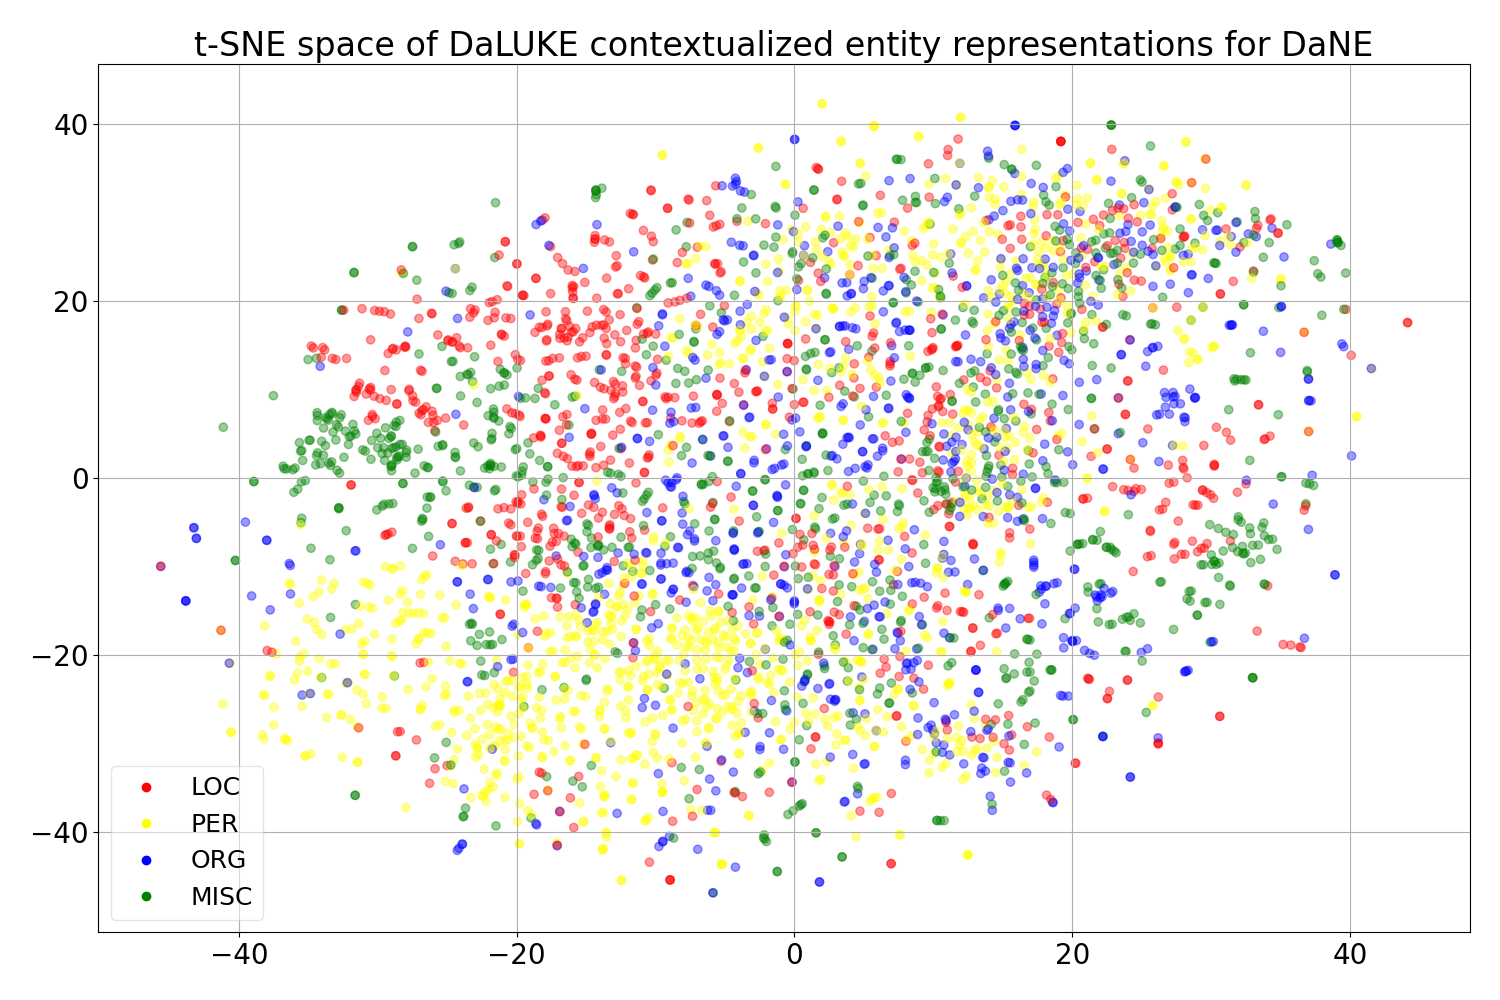
\includegraphics[width=0.495\linewidth]{pos-geo/tsne}
        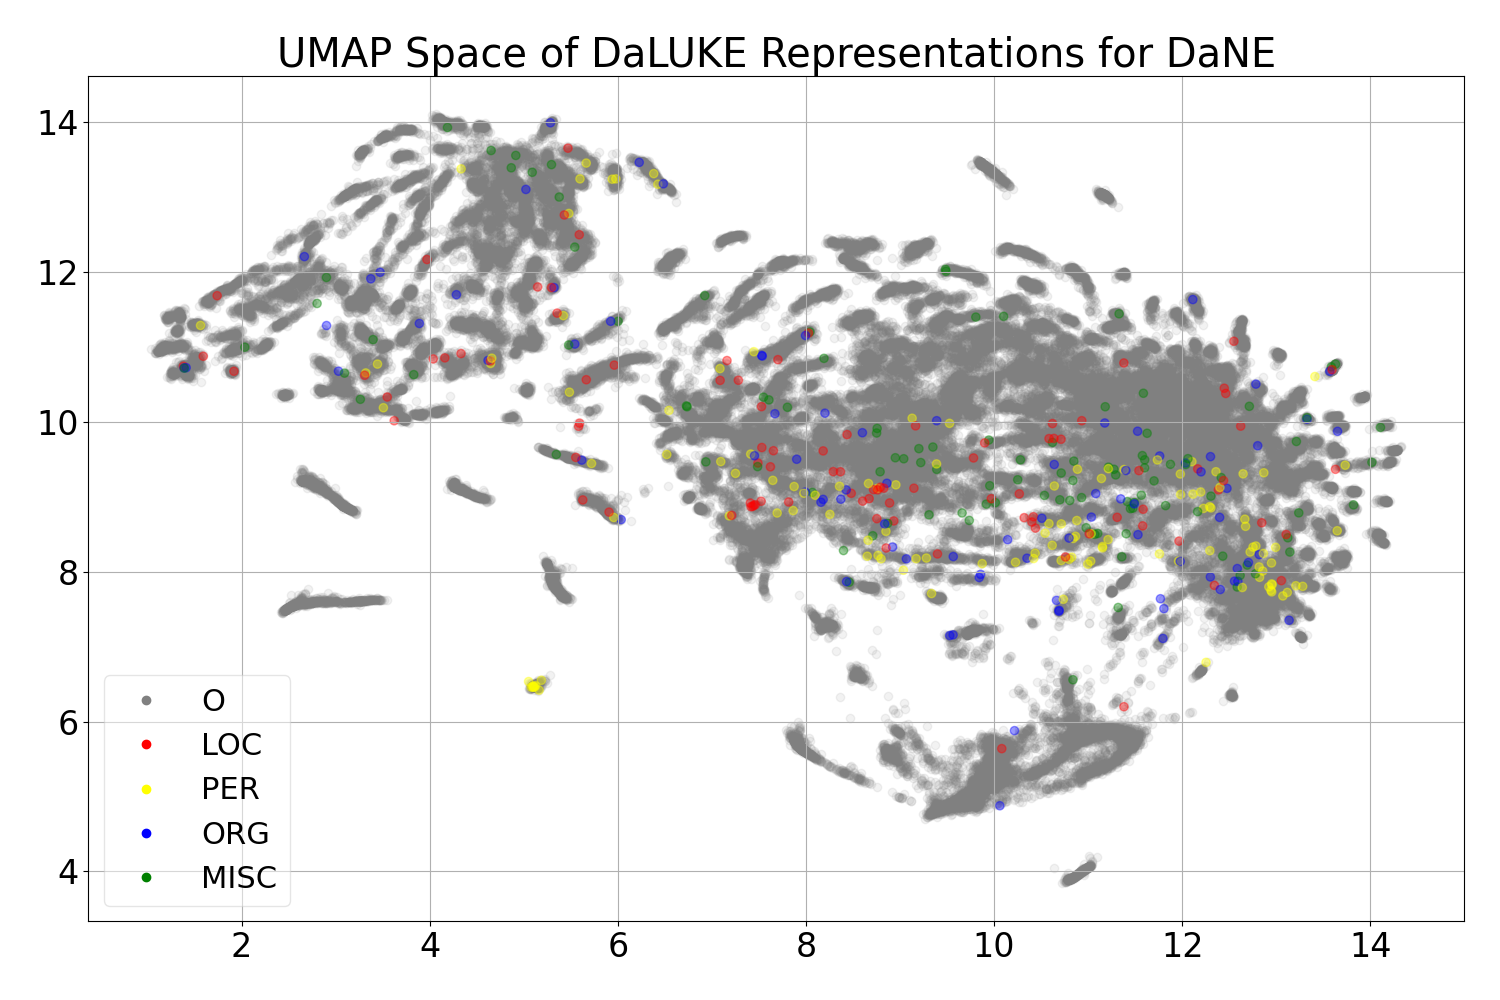
\includegraphics[width=0.495\linewidth]{pos-geo/umap}
    \caption{
        $t$-SNE and UMAP projections of the DaNE dataset containing entity spans with positive labels.
        While the classes are not strongly separated, some clusters consisting of mostly one class are clearly visible in both projections.
    }
    \label{fig:pos-tsne}
\end{figure}\noindent
The obvious question is what these plots mean: What do the clusters and the dimensions themselves correspond to?
This is far from a trivial task; while it is possible to correlate the dimensionality reduced coordinates to the original dimensions, more clever thinking is required to correlate both to human language understanding.
We mostly leave this task for further work, but go through a some of the examples and their projections and present some qualitative observations with supporting examples in Table~\ref{tab:dimexamples}.
\begin{table}[H]
    \footnotesize
    \centering
    \begin{tabularx}{\linewidth}{llclX}
        Data    & Alg.      & Vector                     & \jl{Class}  & Example \\\hline

        Full    & PCA       & $\begin{bmatrix}-11.75\\\underline{36.44}\\-4.85\\16.42\\\vdots\end{bmatrix}$ & O           & De følgende 10 år er der ydet omkring 800 mio. kr. til enkeltprojekter \textbf{og forskningsinstitutter}.\\[3em]

        Full    & PCA       & $\begin{bmatrix}-8.78\\\underline{32.14}\\-1.64\\14.64\\\vdots\end{bmatrix}$ & LOC           & Den syriske leder ankom i går til Abu Dhabi efter besøg i Saudi-Arabien og \textbf{Kuwait}.\\[3em]

        % Full    & PCA       & $\begin{bmatrix}-0.50\\\underline{-11.53}\\-1.78\\5.66\\\vdots\end{bmatrix}$ & O           & Også i Baku \textbf{syntes der at} være roligere, selv om soldater i pansrede køretøjer og lastbiler patruljerede i gaderne, og der var demonstrationer i centrum af byen, oplyste en talsmand for det aserbajdsjanske udenrigsministerium.\\

        Positives    & PCA       & $\begin{bmatrix}-0.23\\-5.63\\-9.60\\\underline{-15.17}\\\vdots\end{bmatrix}$ & MISC        & Det \textbf{jugoslaviske} præsidentråd appellerede i sidste øjeblik til FN om at undlade at iværksætte en boykot og opfordrede til, at der i stedet indkaldes til en international konference om konflikten.\\

        Positives    & PCA       & $\begin{bmatrix}2.30\\5.32\\4.91\\\underline{-13.13}\\\vdots\end{bmatrix}$ & MISC        & Med indsættelse af \textbf{europæiske} fartøjer rykker Vestunionen for første gang i centrum af europæisk sikkerhed efter mange års debat om at lette USAs byrder ved forsvaret af Europa.\\

        Positives    & $t$-SNE       & $\begin{bmatrix}\underline{-37.77}\\-22.41\end{bmatrix}$ & PER        & "Piloten forsøgte at rette maskinen op -- så kunne jeg ikke se mere, men pludselig var der gnister i luften," siger øjenvidnet \textbf{Peter de Neef}.\\

        Positives    & $t$-SNE       & $\begin{bmatrix}\underline{-37.75}\\-22.36\end{bmatrix}$ & PER        & "Løfterne om bonus har jeg heller aldrig fået svar på, hvor bare en undskyldning kunne have gjort underværker," understreger \textbf{Peter Freil}.\\

        Positives    & UMAP       & $\begin{bmatrix}-2.54\\\underline{7.27}\end{bmatrix}$ & MISC       & Datoen for den dag i april, da han fik sin tro på det \textbf{danske} retssystem tilbage.\\

        Positives    & UMAP       & $\begin{bmatrix}-2.07\\\underline{7.17}\end{bmatrix}$ & LOC        & Roskilde Domkirke bliver 12. november rammen om den første af en række koncerter, den norske sangerinde Sissel Kyrkjebø giver i \textbf{Danmark}.

\end{tabularx}
    \caption{
        \footnotesize
        Selected entity examples chosen for having high values in resulting dimensions.
        An example consists of a sentence and an entity candidate -- the example entity span is here visualized with boldface words.
        The coordinate value which is extreme and motivated the inclusion of the example is underlined.
    }
    \label{tab:dimexamples}
\end{table}\noindent
\begin{itemize}
    % TODO: Skal flere understøttende eksempler med i appendiks? - har dem i min local_data
    \item
        The second principal component in the dataset including all data seems to tell something about span position, as the highest values in this dimension almost all correspond to examples with the span at the very end of the sentence.
        Based on this, it makes sense that the plots in Figure~\ref{fig:all-pca} shows the actual entities having moderate values.
    \item
        Low values of the fourth principal component in the positive-label only dataset seems to correspond for a very specific type of words:
        Adjectivizations of political, geographic regions such as "Danish" or "English".
        As explained in Section~\ref{subsec:annoschemes}, such entities should have the label MISC.
        This observation fits with Figure~\ref{fig:pos-pca} showing MISC generally having the lowest 4th dimension values and LOC coming in second.
    \item
        For $t$-SNE on the positive-only data set, no such clear dependencies on coordinate numeric values were observed, explainable by $t$-SNE not returning linear projections, but an approximate recreation of data point distances.
        Two examples very close in $t$-SNE distances are shown in Table~\ref{tab:dimexamples}; these are also semantically very similar in entity type and role.
    \item
        For UMAP fitted to the examples with positive labels, the clear cluster placed around $\begin{bmatrix} -2.5\\ 7\end{bmatrix}$ is examined.
        Here, every entity is revealed to a derivative of the word \emph{Denmark}.
        Some of these are MISC (adjectivizations, demonyms) and some LOC (\emph{Denmark} itself) as seen at Figure~\ref{fig:pos-tsne}.
\end{itemize}
Furthermore, a key quality of the representations is their contextualized nature; this is, superficially, shown to be present in the reduced dimensions, as multiple of these are correlated with the length of the example sequence as shown in Figure~\ref{fig:repvslen}.

\begin{figure}[H]
    \centering
        \includegraphics[width=0.495\textwidth]{full-geo/PCA0-sequence-len}
        \includegraphics[width=0.495\textwidth]{pos-geo/PCA0-sequence-len}
        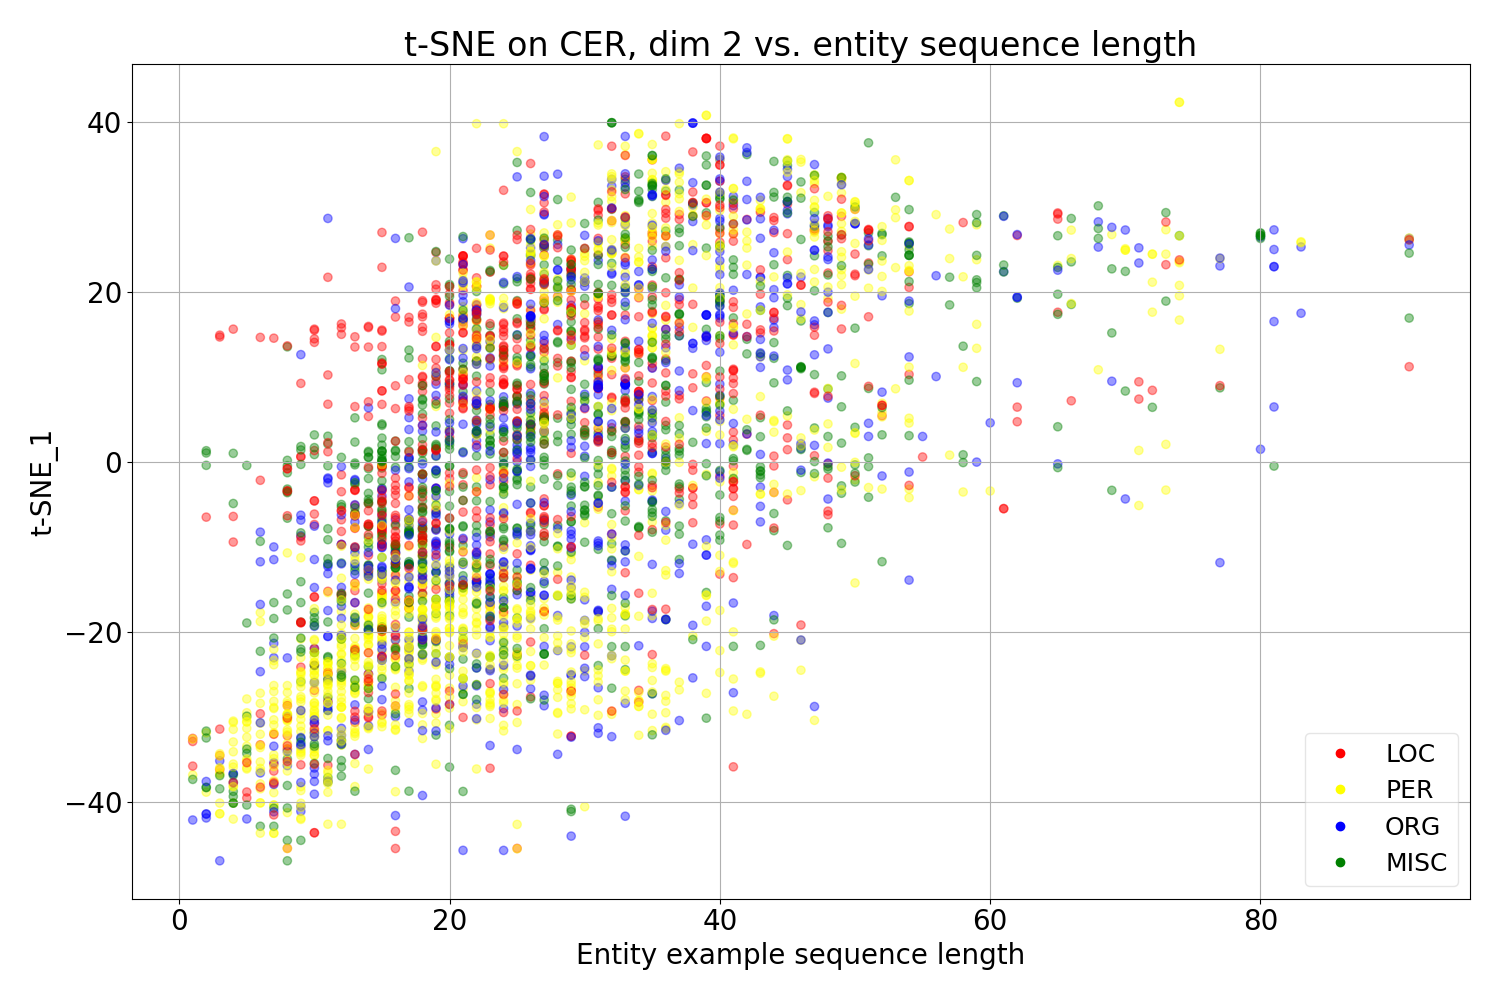
\includegraphics[width=0.495\textwidth]{pos-geo/t-SNE1-sequence-len}
        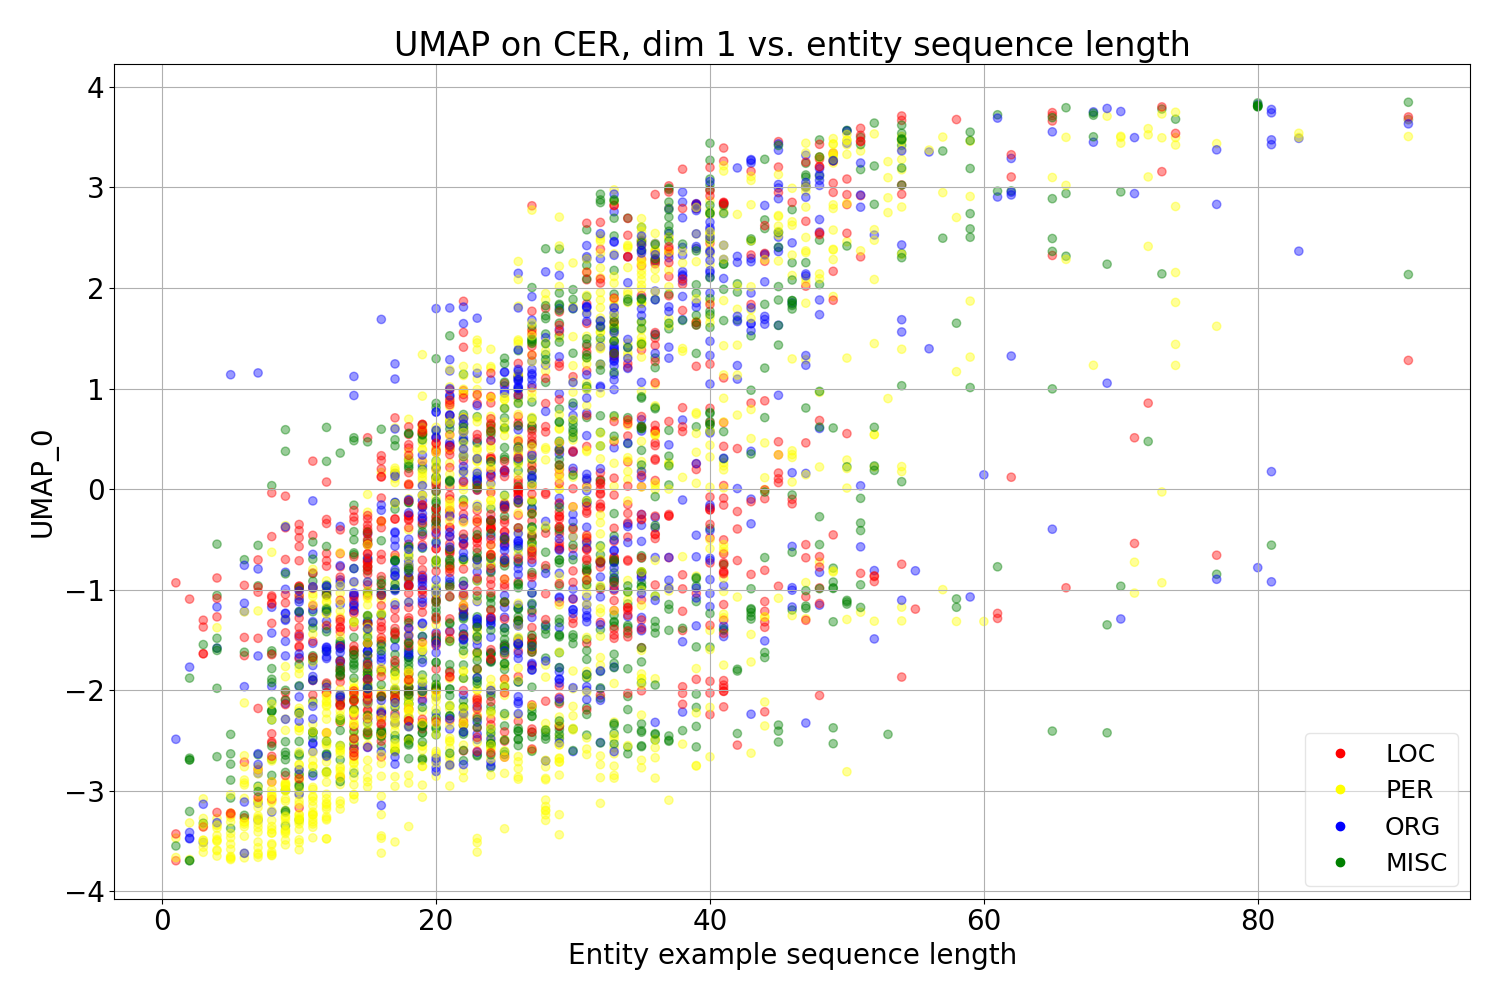
\includegraphics[width=0.495\textwidth]{pos-geo/UMAP0-sequence-len}
     \caption{
        Four selected reduced dimensions, the first (top left) from the full dataset and the three others from the dataset only containing positives, visualized as a function of the length of the sentence that the entity example appears in.
    }
    \label{fig:repvslen}
\end{figure}\noindent

\subsection{When the Model is Wrong}

Analysing when the model is right or wrong may provide valuable insight into how the classification decisions are made and how to improve this.
For this reason, a confusion matrix (table \ref{tab:pred-true-confmat}) is constructed for the DaNE testset that shows predicted labels against the true labels\footnotemark.
\footnotetext{
    All confusion matrices in this section are for simplicity and nuance done on the word level and not on entire entity span level.
    This means that these confusion matrices do not correspond exactly to the reported precision and recall scores, as these were calculated on span level as explained in Section~\ref{sec:nereval}.
}

%      | O    | LOC | PER | ORG | MISC
%-----+------+-----+-----+-----+-----
%O    | 9197 | 5   | 0   | 8   | 14
%LOC  | 5    | 91  | 0   | 2   | 3
%PER  | 5    | 0   | 307 | 3   | 3
%ORG  | 21   | 23  | 11  | 154 | 12
%MISC | 29   | 0   | 0   | 16  | 114

\begin{table}[H]
    \centering
    \small
    \begin{tabular}{l l | r r r r r }
        & &	\multicolumn{5}{c}{Predicted label}	\\
        \multirow{5}{*}{True label} & & LOC & PER & ORG & MISC & O \\\hline
            & LOC  & 91 & 0    & 2   & 3   & 5   \\
            & PER  & 0  & 307  & 2   & 3   & 5   \\
            & ORG  & 23 & 11   & 154 & 12  & 21  \\
            & MISC & 0  & 0    & 16  & 114 & 29  \\
            & O    & 5  & 0    & 8   & 14  & 9,197
    \end{tabular}
    \caption{Predicted labels versus the true labels on the DaNE testset.}
    \label{tab:pred-true-confmat}
\end{table}\noindent
From the table, there are two major sources for errors:
\begin{enumerate}
    \item LOC is often erroneously predicted on ORG entities -- but not the other way around.
    \item O is often predicted on true labels, especially on ORG and MISC. This results in the relatively low recall of $81.18\pro$ holding back performance compared to the precision of $84.67\pro$.
\end{enumerate}
Point 1 may have a relatively simple explanation: 
That many organizations are named after a geographic location while locations more rarely adopts the name of an organization.
Consider for instance the organization entity "Bakken" in the (verbatim) test example: ''Alle som én er en hyldest til Bakken.''.

The model predicts LOC, but while the amusement park, Bakken, would be refer to the physical location in another context, this sentence is about an homage to the spirit or tradition of the park as an institution and is as such marked as ORG.
While the model is contextual meaning correctly predicting such entities is possible, examples with as little context as this one requires a degree of very minute real world knowledge currently not obtained by DaLUKE.
This error pattern also occurred with names of theatres, libraries and municipalities.
For many of these cases, the task is of differentiating between ORG and LOC is further complicated by the fact that the LOC makes up only a subset of the full name.
This means that the model not only has to choose between ORG an LOC for a given entity candidate, but also has to select between a LOC entity and an ORG entity spanning a superset of the LOC span.
If the LOC is the easier prediction, the model will be more confident on that and due to the greedy selection among overlapping spans will not predict ORG.
\begin{table}[H]
    \footnotesize
    \begin{tabular}{l|llllllllll}
        Text:   & Nørrebro  & Bibliotek  & introducerede  &for  &et  &par  &år  &siden  &NU-bøgerne & $\ldots$ \\
        Truth:  & B-ORG     & I-ORG      & O              &O    &O   &O    &O   &O      &B-MISC  & $\ldots$    \\
        Pred.:   & B-LOC     & I-LOC      & O              &O    &O   &O    &O   &O      &O   & $\ldots$\\\hline
    \end{tabular}\par
    \begin{tabular}{l|llllllll}
        Text:    & $\ldots$  &Folkekongressen  &skal  &give  &præsidenten  &diktatoriske  &beføjelser  &.\\
        Truth:   & $\ldots$  &B-ORG            &O     &O     &O            &B-MISC        &O           &O\\
        Pred.:   & $\ldots$  &O                &O     &O     &O            &O             &O           &O\\\hline
    \end{tabular}\par
    \begin{tabular}{l|llllllll}
        Text:    & $\ldots$ &  om  &Landsforeningen  &Ungbo  &har  &begået  &mandatsvig  & $\ldots$ \\
        Truth:   & $\ldots$ &  O   &B-ORG            &I-ORG  &O    &O       &O           & $\ldots$ \\
        Pred.:   & $\ldots$ &  O   &O                &B-ORG  &O    &O       &O           & $\ldots$
    \end{tabular}
    \caption{
        Example sentences where DaLUKE is wrong, including conflating an organization with its location, missing cased and adjective entities, and greedily selecting a subspan instead of the full entity.
    }
    \label{tab:dalukeerrors}
\end{table}\noindent
Point 2, the prevalence of false negatives (prediction case III, following table~\ref{tab:eval}), can be a calibration problem as examined in CALIBRATION, but is also, in our estimation, one of the most difficult parts of this dataset, as the definition of named entities starts becoming quite difficult.
One common cause found is missing a number of adjectives marked as MISC including ''borgerlig'', ''indremissionsk'' and ''olympisk''.
The classification of these as named entities as MISC is correct following CONLL-2003 definition (see Section~\ref{subsec:annoschemes}) but we speculate that this might be a difference in language understanding between English and Danish as this categorization seems non-intuitive in Danish -- in which adjectives are also never capitalized.

In the missed organizations, two possible causes are found.
Firstly, using a case-sensitive tokenizer, which the da-BERT is not \cite{botxo2019dabert}, might help some errors such as ''Markedsudvalget'' and ''Kulturministeriets''.
Secondly, cases such as ''EFs ministerråd'' with the annotation ''B-ORG I-ORG'' are found.
Here, the model only predicts the first word as an organization and gets the entire entity wrong.
As ''EFs'' might follow a pattern more common in the training data than ''EFs ministerråd'', the former has higher estimated probability by the model and is greedily selected.
This tendency to predict subspans highlights a weakness of the method of greedily selecting partially overlapping spans.

From this qualitative impression of the errors, a subset of which are shown in Table~\ref{tab:dalukeerrors}, no smoking gun was found that problematizes this specific model;
contextual understanding and some degree of factural knowledge were exemplifyied for the model in Section~\ref{subsec:mlmpreds}.
Rather, most errors shown here are examples that genuinely are difficult applications of language knowledge.
To get more insight into the prediction patterns of DaLUKE specifically, the NER predictions are compared with those of other Danish NER algorithms.

Initially, the similarity of other model predictions and those of DaLUKE are measured using the proportion of words for which the prediction is the same, shown at Table~\ref{tab:covar}.
Surprisingly, the most similar models are the DaCy models, using the multilingual RoBERTa base and large behind the hood \cite{enevoldsen2020dacy}, and the multilingual BERT from NERDA, while da-BERT, on which DaLUKE is based, follows behind.

\begin{table}[H]
    \centering
    \begin{tabular}{l | c }
        Model               & Same prediction as DaLUKE [\pro]\\\hline
        DaNLP da-BERT       & 97.86\\
        NERDA m-BERT        & 98.44\\
        NERDA Ælæctra       & 97.70\\
        DaCy medium         & 98.68\\
        DaCy large          & \textbf{98.76}\\
        DaNLP spaCy         & 97.65\\
        DaNLP Flair         & 96.37\\
        Polyglot            & 93.45\\
        daner               & 95.90
    \end{tabular}
    \label{tab:covar}
    \caption{
        Covariances between DaLUKE predictions and those of other Danish NER algorithms on the DaLUKE testing dataset.
        This calculation is performed on the word level.
    }
\end{table}\noindent
Compared to the da-BERT predictions, the biggest difference is the higher amount of positive predictions as seen on Table~\ref{tab:dabertcompare}.
DaNLP da-BERT was not finetuned for MISC, so this difference is natural, but DaLUKE also discovers more organizations.
DaLUKE also predicts location more rarely, a class on which DaLUKE outperforms da-BERT (87.0\pro vs. 83.9\pro).

% 2021-06-19 16:31:04.881    INFO        Confusion matrix with DaLUKE results ↓ and results from BERT-DaNE →
% 2021-06-19 16:58:48.906    INFO             | LOC | PER | ORG | MISC | O
%                                        -----+-----+-----+-----+------+-----
%                                        LOC  | 114 | 0   | 0   | 0    | 5
%                                        PER  | 0   | 310 | 5   | 0    | 3
%                                        ORG  | 10  | 9   | 143 | 0    | 21
%                                        MISC | 1   | 0   | 4   | 0    | 141
%                                        O    | 4   | 3   | 6   | 0    | 9244
\begin{table}[H]
    \centering
    \begin{tabular}{l l | r r r r r }
        & &	\multicolumn{5}{c}{da-BERT predictions}	\\
        \multirow{5}{*}{DaLUKE predictions} & & LOC & PER & ORG & MISC & O \\\hline
        & LOC  & 114 & 0   & 0   &  --    & 5  \\
        & PER  & 0   & 310 & 5   &  --    & 3  \\
        & ORG  & 10  & 9   & 143 &  --    & 21 \\
        & MISC & 1   & 0   & 4   &  --    & 141\\
        & O    & 4   & 3   & 6   &  --    & 9244
    \end{tabular}
    \label{tab:dabertcompare}
    \caption{
        da-BERT predictions vs. DaLUKE predictions.
    }
\end{table}\noindent
From examining the examples where the models differ, DaLUKE seems employ the additional learned knowledge to better disambiguate between similar classes and use context to discover named entities, see Table~\ref{tab:daberterrors}.
% Uddybe mere - det her er jo vores chance for at blære

\begin{table}[H]
    \footnotesize
    \begin{tabular}{l|llllllll}
        Text:             & $\ldots$  & redegørelsen  & i  & det    & udenrigspolitiske  & nævn   & $\ldots$ \\
        Truth:            & $\ldots$  & O             & O  & B-ORG  & I-ORG              & I-ORG  & $\ldots$ \\\hline
        DaLUKE pred.:     & $\ldots$  & O             & O  & B-ORG  & I-ORG              & I-ORG  & $\ldots$ \\
        da-BERT pred.:    & $\ldots$  & O             & O  & O      & O                  & O      & $\ldots$ \\
    \end{tabular}\par
    \begin{tabular}{l|lllllllllllllll}
        Text:            &  "Ih,   & hvor  & jeg  & glæder  & mig  & til  & et  & lille  & glas,"  & lød  & det  & fra  & Lykke  \\
        Truth:           &  O    & O     & O    & O       & O    & O    & O   & O      & O        & O    & O    & O    & B-PER  \\\hline
        DaLUKE pred.:    &  O    & O     & O    & O       & O    & O    & O   & O      & O        & O    & O    & O    & B-PER  \\
        da-BERT pred.:   &  O    & O     & O    & O       & O    & O    & O   & O      & O        & O    & O    & O    & O
    \end{tabular}\par
    \begin{tabular}{l|llllllllllll}
        Text:            & Rapporten  & $\ldots$  & er  & bestilt  & og  & betalt  & af  & Københavns  & Amtsråd  & $\ldots$\\
        Truth:           & O          & $\ldots$  & O   & O        & O   & O       & O   & B-ORG       & I-ORG    & $\ldots$\\\hline
        DaLUKE  pred.:   & O          & $\ldots$  & O   & O        & O   & O       & O   & B-ORG       & I-ORG    & $\ldots$\\
        da-BERT pred.:   & O          & $\ldots$  & O   & O        & O   & O       & O   & B-LOC       & I-LOC    & $\ldots$
    \end{tabular}
    \caption{
    }
    \label{tab:daberterrors}
\end{table}\noindent
The same comparison is made to DaCy Large which achieves higher performance than DaLUKE -- especially driven by improvements in organization and miscellaneous classes.
Here, the biggest differences lies in cases where the models have to discern between these two classes and  null class, seen at Table~\ref{tab:dacycompare}.

% 2021-06-19 16:29:26.614    INFO        Confusion matrix with DaLUKE results ↓ and results from DaCyLarge-DaNE →
% 2021-06-19 16:58:11.740    INFO             | LOC | PER | ORG | MISC | O
%                                        -----+-----+-----+-----+------+-----
%                                        LOC  | 108 | 0   | 2   | 1    | 8
%                                        PER  | 0   | 309 | 6   | 3    | 0
%                                        ORG  | 9   | 3   | 154 | 5    | 12
%                                        MISC | 0   | 1   | 3   | 120  | 22
%                                        O    | 8   | 4   | 8   | 27   | 9210
\begin{table}[H]
    \centering
    \begin{tabular}{l l | r r r r r }
        & &	\multicolumn{5}{c}{DaCy Large predictions}	\\
        \multirow{5}{*}{DaLUKE predictions} & & LOC & PER & ORG & MISC & O \\\hline
           & LOC                             &  108 & 0   & 2   & 1    & 8\\
           & PER                             &  0   & 309 & 6   & 3    & 0\\
           & ORG                             &  9   & 3   & 154 & 5    & 12\\
           & MISC                            &  0   & 1   & 3   & 120  & 22\\
           & O                               &  8   & 4   & 8   & 27   & 9210
    \end{tabular}
    \label{tab:dacycompare}
    \caption{
        DaCy Large predictions vs. DaLUKE predictions.
    }
\end{table}\noindent
Examples where DaCy is right, but DaLUKE wrong is shown at Table~\ref{tab:dacyex}.
These give more possible causes of the improvement, adding to the initial explanation of DaCy employing a BERT \emph{large}-sized transformer, adding flexibility to the model, theoretically allowing higher level language features to be learned compared to the base size model used by DaLUKE.
One cause is the use of the case sensitive byte-pair encoding tokenizer of RoBERTa \cite{conneau2020unsupervised} which we speculate helps discovering more entities, relating to the high recall of DaCy (83.7\pro versus the 81.2\pro of DaLUKE).
Another interesting pattern lies in the strength of the multilingual model used by DaCy correctly predicting entities in foreign languages.

\begin{table}[H]
    \footnotesize
    \begin{tabular}{l|llllll}
        Text:             & $\ldots$  & opus    & VIII    & der  & hedder  \\
        Truth:            & $\ldots$  & B-MISC  & I-MISC  & O    & O       \\\hline
        DaLUKE pred.:     & $\ldots$  & B-MISC  & I-MISC  & O    & O       \\
        DaCy pred.:       & $\ldots$  & O       & O       & O    & O       
    \end{tabular}
    (continued)\\
    \begin{tabular}{c} % The spooky, scary, invisible ghost table for formatting!
        \quad \quad \quad \quad \quad \quad \quad \quad \quad \quad \quad \quad \quad \quad \quad \quad \quad \quad 
    \end{tabular}
                \begin{tabular}{llllll}
                     Il      & Cimento  & dell'Armonia  & e       & dell'Invenzione \\
                     B-MISC  & I-MISC   & I-MISC        & I-MISC  & I-MISC          \\\hline
                     O       & O        & O             & O       & O               \\
                     B-MISC  & I-MISC   & I-MISC        & I-MISC  & I-MISC          
                \end{tabular}\par
    \begin{tabular}{l|llllllll}
        Text:             & Der  & ligger  & fire  & skodder  & plus  & en  & hel  & Camel   \\ 
        Truth:            & O    & O       & O     & O        & O     & O   & O    & B-MISC  \\\hline
        DaLUKE pred.:     & O    & O       & O     & O        & O     & O   & O    & O       \\ 
        DaCy pred.:    & O    & O       & O     & O        & O     & O   & O    & B-MISC
    \end{tabular}\par
    \begin{tabular}{l|llllllllll}
        Text:            & Den  & modtog  & han  & i  & øvrigt  & Kulturministeriets  & børnebogspris  & for  & i  & 1990 \\
        Truth:           & O    & O       & O    & O  & O       & B-ORG               & O              & O    & O  & O    \\\hline
        DaLUKE  pred.:   & O    & O       & O    & O  & O       & O                   & O              & O    & O  & O    \\
        DaCy pred.:   & O    & O       & O    & O  & O       & B-ORG               & O              & O    & O  & O    
    \end{tabular}
    \caption{
    }
    \label{tab:dacyex}
\end{table}\noindent

\section{Summary}
%TODO Bedre navn, så 6.1.8 ikke gentages


\end{document}
